%==================================
% SMDS TEMPLATE (VERSI BAHASA INDONESIA)
%==================================
\documentclass[11pt,twoside]{article}

\usepackage{titlesec}
\titlespacing*{\section}{0pt}{1.5ex plus 0.5ex minus 0.2ex}{0.8ex plus 0.2ex}
\titlespacing*{\subsection}{0pt}{1.2ex plus 0.5ex minus 0.2ex}{0.5ex plus 0.2ex}

\usepackage[utf8]{inputenc}
\usepackage{amsmath,amssymb}
\usepackage[T1]{fontenc}
\usepackage{lmodern}
\usepackage{graphicx}
\usepackage{geometry}
\geometry{margin=1in}
\usepackage{booktabs}
\usepackage{array}
\usepackage{tabularx}
\usepackage{longtable}
\usepackage{adjustbox}
\usepackage{float}
\usepackage{caption}
\usepackage{placeins}
\usepackage{subcaption}
\usepackage{csquotes}
\usepackage[
backend=biber,
style=numeric-comp,
sorting=none,
giveninits=true,
doi=true,
url=true
]{biblatex}
\addbibresource{SMDSBib.bib}
\usepackage{fancyhdr}
\newcommand{\shorttitle}{}
\newcommand{\shortauthor}{}
\pagestyle{fancy}
\fancyhf{}
\fancyhead[L]{\small\shorttitle}
\fancyhead[R]{\small\shortauthor}
\fancyfoot[C]{\thepage}

\usepackage[colorlinks=true,allcolors=blue]{hyperref}
\newcommand{\orcidlink}[1]{%
\href{https://orcid.org/#1}{
\includegraphics[height=1.6ex]{ORCID_iD.png}}%
}

\graphicspath{{figures/}}
\captionsetup{font=small,labelfont=bf}
\setlength{\parindent}{1.2em}
\setlength{\parskip}{0.25em}
\sloppy

\newcommand{\SMDStitle}[1]{\title{\bfseries #1}}
\newcommand{\SMDSshorttitle}[1]{\def\shorttitle{#1}}
\newcommand{\SMDSshortafill}[1]{\def\shortauthor{#1}}

\newcommand{\SMDSaffilone}[1]{\def\affilone{#1}}
\newcommand{\SMDSauthorone}[4]{\def\authorone{#1$^{#2}$\,\orcidlink{#3}}}
\newcommand{\SMDSauthortwo}[4]{\def\authortwo{#1$^{#2}$\,\orcidlink{#3}}}

\newcommand{\SMDScorrespoding}[2]{%
\def\corrauthor{#1 \href{mailto:#2}{#2}}}

\newcommand{\SMDSKeywords}[1]{
\vspace{0.5em}
\noindent\textbf{Kata Kunci:} #1
}

\newcommand{\acknowledg}[1]{
\section*{Ucapan Terima Kasih}
#1
}

%==================================
% METADATA
%==================================

\SMDStitle{Analisis Sensitivitas Produk Elevasi Global terhadap Pemetaan Kerawanan Banjir Berbasis \textit{Machine Learning} Menggunakan Google Earth Engine: Studi Komparatif Terkontrol SRTM, Copernicus DEM GLO-30, dan ALOS AW3D30 di Wilayah Pesisir Semarang--Demak}

\SMDSshortafill{M. I. A. Hakim and A. G. Z. Fann}
\SMDSshorttitle{Sensitivitas DEM Global pada Pemetaan Kerawanan Banjir}

\SMDSaffilone{Program Studi Statistika dan Sains Data, Fakultas Matematika dan Ilmu Pengetahuan Alam, Universitas Negeri Semarang, Indonesia}

\SMDSauthorone{M Irfan Al Hakim}{1}{0009-0005-1222-7960}
{mirfanhakim25@students.unnes.ac.id}

\SMDSauthortwo{Alverrell Gustivierda Zidna Fann}{1}{0009-0002-5764-3229}
{alverrell@students.unnes.ac.id}

\SMDScorrespoding{$^*$Penulis korespondensi, email:}{%
    mirfanhakim25@students.unnes.ac.id;
}

\author{
\begin{minipage}{\textwidth}
\authorone,
\authortwo
\\[1em]
$^1$ \affilone\\
\corrauthor
\end{minipage}
}

\date{\vspace{-1.5em}}
\begin{document}

\maketitle

\begin{abstract}
Produk \textit{Digital Elevation Model} (DEM) global beresolusi 30 meter banyak digunakan sebagai sumber topografi utama dalam pemetaan kerawanan banjir (\textit{flood susceptibility mapping}) berbasis \textit{machine learning} ketika data LiDAR beresolusi tinggi tidak tersedia. Namun, perbedaan karakteristik sensor, penetrasi kanopi, serta acuan geoid vertikal antarproduk berpotensi menghasilkan variasi representasi permukaan yang merambat hingga ke prediksi spasial. Penelitian ini mengukur sensitivitas pemetaan kerawanan banjir berbasis Random Forest terhadap pemilihan tiga produk elevasi global---SRTM, Copernicus DEM GLO-30, dan ALOS AW3D30---di wilayah pesisir Semarang--Demak, Jawa Tengah. Menggunakan desain eksperimen terkontrol satu faktor pada Google Earth Engine dan Python, kami mengunci identik \textit{flood inventory} Sentinel-1 SAR (kejadian banjir Maret 2024), 19 prediktor lingkungan non-DEM dan tutupan lahan, sampel induk berimbang ($n = 5.956$; 2.978 titik banjir dan 2.978 titik non-banjir), pembagian data latih--uji, serta parameter Random Forest, dengan hanya memvariasikan lima prediktor topografi turunan DEM (elevasi, kemiringan lereng, komponen sinus dan kosinus arah lereng, serta indikator validitas arah lereng). Hasil empiris menunjukkan bahwa ketiga konfigurasi DEM menghasilkan daya diskriminasi yang tinggi baik pada evaluasi \textit{holdout} acak terstratifikasi ($\text{ROC-AUC} = 0{,}932\text{--}0{,}940$) maupun validasi silang spasial 4-\textit{fold} pada 16 blok kuantil koordinat ($\text{ROC-AUC} = 0{,}870\text{--}0{,}890$). Pengujian \textit{block bootstrap} berpasangan (1.000 iterasi pada 16 blok) mengonfirmasi keunggulan kecil namun konsisten dari Copernicus DEM GLO-30 terhadap SRTM ($\Delta\text{AUC}_{\text{SRTM}-\text{GLO-30}} = -0{,}0155$, CI 95\% $[-0{,}0250; -0{,}0072]$) dan ALOS AW3D30 ($\Delta\text{AUC}_{\text{GLO-30}-\text{AW3D30}} = +0{,}0108$, CI 95\% $[+0{,}0041; +0{,}0198]$), sedangkan SRTM dan ALOS AW3D30 tidak berbeda signifikan secara statistik ($\Delta\text{AUC} = -0{,}0047$, CI 95\% $[-0{,}0096; +0{,}0013]$). Pengulangan menyeluruh lintas lima \textit{seed} independen membuktikan kestabilan urutan peringkat ($\text{Spatial-CV AUC} = 0{,}889 \pm 0{,}013$ untuk GLO-30 vs.\ $0{,}877 \pm 0{,}017$ untuk AW3D30 dan $0{,}869 \pm 0{,}017$ untuk SRTM). Meskipun selisih metrik agregat tergolong kecil, perbandingan pasca-masking AOI ($1{,}44 \times 10^6$ piksel valid) mengungkap kesesuaian lima kelas sebesar 79,4\%--84,3\%, pergeseran luas Kelas 5 ($p > 0{,}80$) dari $100{,}58\text{ km}^2$ (SRTM) menjadi $95{,}93\text{ km}^2$ (AW3D30, $-4{,}6\%$) dan $109{,}63\text{ km}^2$ (GLO-30, $+9{,}0\%$) yang terkonsentrasi pada semak belukar (57,6\%--75,4\%), mangrove (62,6\%--74,9\%), dan lahan pertanian (69,3\%--75,5\%), serta autokorelasi Global Moran's $I$ signifikan pada residual \textit{out-of-fold} ($0{,}355\text{--}0{,}377$, $p = 0{,}0001$).
\end{abstract}

\SMDSKeywords{pemetaan kerawanan banjir, sensitivitas Digital Elevation Model, SRTM, Copernicus DEM GLO-30, ALOS AW3D30, Random Forest, validasi silang blok spasial, Semarang--Demak}

%==================================
\section{Pendahuluan}\label{sec:pendahuluan}

Pemetaan kerawanan banjir (\textit{flood susceptibility mapping}) bertujuan mengestimasi kecenderungan spasial suatu bentang lahan untuk mengalami genangan berdasarkan faktor pengondisi topografi, hidrologi, meteorologi, dan karakteristik permukaan. Karena interaksi antarvariabel lingkungan bersifat nonlinier, algoritma \textit{ensemble machine learning}---khususnya Random Forest \cite{breiman2001}---telah menjadi pendekatan utama dalam pemodelan kerawanan banjir regional \cite{saha2021,avand2022,hakim2026}. Di kawasan pesisir dataran rendah yang tidak memiliki survei topografi LiDAR (\textit{Light Detection and Ranging}) maupun peta genangan lapangan beresolusi tinggi, alur kerja pemetaan sangat bergantung pada data satelit terbuka yang diolah melalui platform komputasi awan seperti Google Earth Engine (GEE) \cite{gorelick2017}.

Salah satu komponen paling mendasar dalam alur kerja berbasis data terbuka tersebut adalah pemilihan produk \textit{Digital Elevation Model} (DEM) global. Pada skala resolusi 30 meter, terdapat tiga produk elevasi global yang paling luas digunakan: SRTM (\textit{Shuttle Radar Topography Mission}) yang diturunkan dari interferometri radar pita-C \cite{farr2007}, Copernicus DEM GLO-30 yang berasal dari interferometri radar bistatik pita-X misi TanDEM-X \cite{esa_glo30}, serta ALOS AW3D30 (\textit{ALOS World 3D 30m}) yang direkonstruksi secara fotogrametrik dari citra stereo optik sensor PRISM \cite{tadono2016}. Walaupun ketiganya memiliki ukuran piksel nominal yang sebanding (30 meter), ketiganya berasal dari teknik penginderaan, periode akuisisi, karakteristik interaksi kanopi/bangunan, dan datum geoid vertikal yang berbeda (EGM96 pada SRTM dan ALOS AW3D30 berbanding EGM2008 pada Copernicus GLO-30). Evaluasi global oleh Meadows dkk.\ \cite{meadows2024} terhadap 65 survei LiDAR di kawasan rawan banjir membuktikan bahwa galat vertikal produk DEM global bervariasi secara sistematis menurut kemiringan lereng dan kelas tutupan lahan, sehingga tidak ada satu pun produk DEM global yang secara universal paling unggul di seluruh kondisi lingkungan.

Sejumlah studi terbaru telah menyoroti pengaruh pemilihan atau resolusi DEM terhadap pemodelan banjir \cite{ali2015,fatdillah2022,fereshtehpour2024,adesina2025,fikri2026,salgado2026}. Pada pemetaan \textit{flood susceptibility} berbasis data terbuka di Nigeria, Tique dkk.\ \cite{Tique2026} membandingkan empat produk DEM, beberapa metode delineasi hidrologi, dan tiga algoritma \textit{machine learning}. Namun, ketika desain penelitian mengubah produk DEM, metode hidrologi, dan algoritma pemodelan secara bersamaan, kontribusi spesifik dari sumber data elevasi tidak dapat dipisahkan secara murni dari variasi algoritmik.

Dalam penelitian acuan kami sebelumnya di jurnal \textit{Statistical Modeling and Data Science} (SMDS) \cite{hakim2026}, kami membangun kerangka pemetaan kerawanan banjir di kawasan pesisir Semarang--Demak dengan mengintegrasikan \textit{flood inventory} berbasis deteksi perubahan Sentinel-1 SAR dan tujuh model \textit{ensemble learning}. Studi acuan tersebut menunjukkan bahwa Random Forest mencapai daya diskriminasi titik tertinggi ($\text{ROC-AUC} = 0{,}852$). Melanjutkan studi tersebut, artikel ini menggeser fokus dari \emph{komparasi algoritma} menuju \emph{eksperimen sensitivitas sumber data elevasi yang terkontrol}. Random Forest ditetapkan sebagai model yang dikontrol, sementara batas wilayah, \textit{flood inventory} Sentinel-1, prediktor non-DEM, lokasi titik sampel, dan parameter model dipertahankan identik, sehingga produk elevasi global (SRTM, Copernicus DEM GLO-30, dan ALOS AW3D30) menjadi satu-satunya faktor perlakuan.

Kawasan pesisir Semarang--Demak merupakan laboratorium alami yang sangat relevan untuk menguji sensitivitas DEM karena morfologi dataran aluvialnya yang sangat landai berinteraksi dengan jaringan sungai, tambak, lahan pertanian, kawasan terbangun, serta penurunan muka tanah yang intensif \cite{marfai2008,abidin2015,Husnayaen2018,yuwono2024,verdyansyah2025,Sakina2025}. Di samping itu, untuk menghindari bias optimisme akibat autokorelasi spasial pada pembagian data acak \cite{roberts2017,ploton2020}, evaluasi penelitian ini dilengkapi dengan validasi silang spasial berbasis blok, \textit{block bootstrap} berpasangan, serta pengujian ketahanan lintas lima nilai \textit{seed}.

Secara spesifik, penelitian ini menjawab empat rumusan masalah: (1) sejauh mana perbedaan karakteristik SRTM, Copernicus DEM GLO-30, dan ALOS AW3D30 tercermin pada parameter topografi turunan di wilayah pesisir Semarang--Demak; (2) bagaimana pengaruh pergantian sumber elevasi terhadap kinerja prediktif dan peta probabilitas Random Forest dalam eksperimen terkontrol; (3) seberapa sensitif metrik evaluasi dan distribusi spasial kelas kerawanan ketika autokorelasi spasial diperhitungkan melalui validasi blok dan \textit{block bootstrap}; serta (4) apakah sensitivitas spasial antarpeta menunjukkan pola yang berbeda antar kelas tutupan lahan ESA WorldCover.

\begin{table}[!htbp]
\small
\centering
\caption{Posisi eksperimen terkontrol penelitian ini terhadap studi terdahulu terkait DEM dan pemetaan kerawanan banjir.}
\label{tab:prior-studies-id}
\begin{adjustbox}{max width=\textwidth}
\begin{tabular}{>{\raggedright}p{3.0cm} >{\raggedright}p{3.6cm} >{\raggedright}p{3.8cm} >{\raggedright\arraybackslash}p{4.4cm}}
\toprule
\textbf{Penelitian} & \textbf{Fokus Utama} & \textbf{Konsep yang Diadopsi} & \textbf{Pengembangan pada Penelitian Ini} \\
\midrule
Fatdillah dkk.\ (2022) \cite{fatdillah2022}; Fikri dkk.\ (2026) \cite{fikri2026} & Pengaruh resolusi dan sumber DEM pada pemodelan hidrolika banjir & Variasi input topografi merambat ke estimasi risiko banjir & Diuji dalam kerangka \textit{machine learning} terkontrol satu faktor \\
Meadows dkk.\ (2024) \cite{meadows2024} & Evaluasi akurasi vertikal DEM global 30\,m terhadap 65 survei LiDAR & Galat SRTM, Copernicus GLO-30, dan AW3D30 bergantung pada lereng dan tutupan lahan & Dampak perbedaan DEM ditelusuri hingga peta kerawanan spasial dan stratifikasi WorldCover \\
Yuwono dkk.\ (2024) \cite{yuwono2024}; Verdyansyah dkk.\ (2025) \cite{verdyansyah2025} & Pemodelan bahaya dan kerawanan banjir di Semarang dan Demak & Konteks fisik banjir pesisir dan faktor pengondisi lokal & Memvariasikan sumber DEM global secara sistematis dengan model terkontrol \\
Hakim dkk.\ (2026) \cite{hakim2026} & \textit{Flood inventory} Sentinel-1 + 7 model \textit{ensemble} di Semarang--Demak & Protokol label Sentinel-1 dan baseline Random Forest & Mengunci Random Forest, mengisolasi perlakuan DEM, serta mengoreksi bias domain sampel JRC \\
Tique dkk.\ (2026) \cite{Tique2026} & Komparasi multi-DEM, multi-hidrologi, dan multi-ML di Nigeria & Bukti empiris bahwa pilihan DEM mengubah pemetaan kerawanan banjir & Mengontrol algoritma, label, dan prediktor non-DEM agar efek sumber DEM terisolasi murni \\
\bottomrule
\end{tabular}
\end{adjustbox}
\end{table}

%==================================
\section{Wilayah Studi dan Data}\label{sec:wilayah-data}

\subsection{Wilayah Penelitian}\label{subsec:wilayah}

Wilayah kajian (\textit{Area of Interest}/AOI) mencakup Kota Semarang dan Kabupaten Demak di pesisir utara Jawa Tengah berdasarkan batas administrasi FAO GAUL Level 2 ($110{,}27^\circ\text{BT}\text{--}110{,}83^\circ\text{BT}$, $7{,}14^\circ\text{LS}\text{--}6{,}71^\circ\text{LS}$). Pada grid analisis seragam 30 meter dalam proyeksi UTM Zona 49S (\texttt{EPSG:32749}), wilayah kajian mencakup $1.469.555$ piksel grid pra-masking dan, setelah masking batas poligon AOI (\texttt{FAO/GAUL/2015/level2} Kabupaten Demak dan Kota Semarang, luas geodesik $1.310{,}09\text{ km}^2$), mencakup $1.444.085$ piksel valid ($1.299{,}84\text{ km}^2$ sferis / $1.299{,}68\text{ km}^2$ planar) pada SRTM dan Copernicus GLO-30 serta $1.429.582$ piksel valid ($1.286{,}79\text{ km}^2$ sferis / $1.286{,}62\text{ km}^2$ planar) pada ALOS AW3D30. Secara morfologis, wilayah ini terbagi atas dataran aluvial pesisir utara yang sangat datar (elevasi umumnya $<5\text{ m}$ dengan lereng $<2^\circ$) dan perbukitan kaki gunung api di bagian selatan Kota Semarang yang mencapai ketinggian $>230\text{ m}$ \cite{marfai2008,abidin2015,Husnayaen2018}.

\subsection{Produk Elevasi Perlakuan dan Dataset Geospasial Multi-Sumber}\label{subsec:data}

Seluruh dataset geospasial diakuisisi dan diselaraskan pada Google Earth Engine \cite{gorelick2017} menggunakan grid 30 meter \texttt{EPSG:32749} (Tabel~\ref{tab:data-id}). Tiga produk elevasi global beresolusi 30 meter yang diuji sebagai faktor perlakuan adalah:
\begin{enumerate}
\item \textbf{SRTM (\texttt{USGS/\allowbreak SRTMGL1\_003})} \cite{farr2007}: Diukur melalui interferometri radar pita-C ($\lambda \approx 5{,}6\text{ cm}$) pada misi STS-99 tahun 2000 dengan datum geoid vertikal EGM96. Pantulan sebagian sinyal pita-C oleh tajuk vegetasi dan atap bangunan membuat SRTM berkarakteristik mendekati \textit{Digital Surface Model} (DSM).
\item \textbf{Copernicus DEM GLO-30 (\texttt{COPERNICUS/\allowbreak DEM/\allowbreak GLO30})} \cite{esa_glo30}: Diturunkan dari interferometri radar bistatik pita-X ($\lambda \approx 3{,}1\text{ cm}$) lintasan tunggal misi TanDEM-X dengan datum vertikal EGM2008.
\item \textbf{ALOS AW3D30 v4.1 (\texttt{JAXA/\allowbreak ALOS/\allowbreak AW3D30/\allowbreak V4\_1})} \cite{tadono2016}: Dihasilkan dari rekonstruksi fotogrametri stereo optik pankromatik sensor PRISM dengan datum vertikal EGM96 (setara dengan SRTM, sedangkan Copernicus GLO-30 mengacu pada EGM2008). Pita \textit{void mask} resmi (\texttt{MSK}) dievaluasi secara eksplisit di wilayah kajian: piksel observasi valid ($\texttt{MSK}=0$) mencakup $1.292{,}84\text{ km}^2$ ($99{,}1\%$), sedangkan piksel pengisian awan/void ($\texttt{MSK}=3$ dan $48$) hanya mencakup $1{,}44\text{ km}^2$ dan $10{,}07\text{ km}^2$; pemodelan mempertahankan piksel valid $\texttt{MSK}=0$.
\end{enumerate}

\begin{table}[!htbp]
\small
\centering
\caption{Matriks data penelitian, resolusi spasial, ID katalog Google Earth Engine, dan fungsi analitis.}
\label{tab:data-id}
\begin{adjustbox}{max width=\textwidth}
\begin{tabular}{>{\raggedright}p{2.7cm} >{\raggedright}p{2.8cm} >{\raggedright}p{1.6cm} >{\raggedright}p{4.3cm} >{\raggedright\arraybackslash}p{3.4cm}}
\toprule
\textbf{Dataset} & \textbf{Jenis / Sifat Sensor} & \textbf{Resolusi Asli} & \textbf{Produsen \& ID Katalog GEE} & \textbf{Fungsi dalam Eksperimen} \\
\midrule
Sentinel-1 GRD & Radar SAR pita-C (VH, dB) & 10\,m (IW) & ESA Copernicus; \texttt{COPERNICUS/\allowbreak S1\_GRD} & \textit{Flood inventory} biner terkunci (Maret 2024) \\
SRTM GL1 v3 & InSAR pita-C DSM (EGM96, m) & 30\,m & NASA/USGS; \texttt{USGS/\allowbreak SRTMGL1\_003} & Perlakuan Elevasi 1 (5 prediktor topografi) \\
Copernicus DEM GLO-30 & InSAR bistatik pita-X DSM (EGM2008, m) & 30\,m & ESA Copernicus; \texttt{COPERNICUS/\allowbreak DEM/\allowbreak GLO30} & Perlakuan Elevasi 2 (5 prediktor topografi) \\
ALOS AW3D30 v4.1 & Stereo optik PRISM DSM (EGM96, m) & 30\,m & JAXA; \texttt{JAXA/\allowbreak ALOS/\allowbreak AW3D30/\allowbreak V4\_1} & Perlakuan Elevasi 3 (5 prediktor topografi) \\
MERIT Hydro v1.0.1 & Hidrografi terkondisi DEM & 90\,m & Univ.\ Tokyo \cite{yamazaki2019}; \texttt{MERIT/\allowbreak Hydro/\allowbreak v1\_0\_1} & Prediktor hidrologi terkunci (\texttt{hand}, \texttt{upa\_log}, \texttt{river\_width}, \texttt{dist\_river}) \\
JRC Global Surface Water & Frekuensi air permukaan (1984--2021, \%) & 30\,m & EC JRC \cite{pekel2016}; \texttt{JRC/\allowbreak GSW1\_4/\allowbreak Global\allowbreak SurfaceWater} & Masking air permanen ($\ge 80\%$) \& \texttt{dist\_perm\_water} \\
CHIRPS Daily & Presipitasi IR + stasiun (mm) & $0{,}05^\circ$ ($\sim$5,5\,km) & UCSB CHG \cite{funk2015}; \texttt{UCSB-CHG/\allowbreak CHIRPS/\allowbreak DAILY} & Curah hujan antecedent 7 \& 30 hari terkunci \\
Sentinel-2 SR (L2A) & Reflektansi permukaan optik & 10--20\,m & ESA Copernicus; \texttt{COPERNICUS/\allowbreak S2\_SR\_\allowbreak HARMONIZED} & Indeks spektral terkunci (\texttt{ndvi}, \texttt{ndwi}, \texttt{mndwi}, \texttt{ndbi}) \\
ESA WorldCover v200 & Klasifikasi tutupan lahan (2021) & 10\,m & ESA \cite{zanaga2021}; \texttt{ESA/\allowbreak WorldCover/\allowbreak v200} & Variabel \textit{dummy} terkunci + stratifikasi spasial \\
\bottomrule
\end{tabular}
\end{adjustbox}
\end{table}

%==================================
\section{Metodologi}\label{sec:metodologi}

\subsection{Desain Eksperimen Terkontrol Satu Faktor}\label{subsec:desain-eksperimen}

Untuk mengisolasi pengaruh sumber produk elevasi secara murni, penelitian ini menerapkan desain eksperimen terkontrol dengan tiga level perlakuan: SRTM, Copernicus DEM GLO-30, dan ALOS AW3D30 (Tabel~\ref{tab:desain-id}). Seluruh komponen di luar prediktor turunan DEM dikunci identik di ketiga perlakuan, meliputi label banjir Sentinel-1, batas AOI dan grid 30\,m \texttt{EPSG:32749}, 19 prediktor non-DEM, koordinat titik sampel induk ($n=5.956$), pembagian latih--uji serta blok spasial, hingga konfigurasi hiperparameter Random Forest.

\begin{table}[!htbp]
\small
\centering
\caption{Rancangan eksperimen terkontrol untuk menguji sensitivitas sumber produk elevasi global.}
\label{tab:desain-id}
\begin{tabular}{>{\raggedright}p{4.5cm} >{\raggedright\arraybackslash}p{9.8cm}}
\toprule
\textbf{Komponen Eksperimen} & \textbf{Spesifikasi pada Ketiga Perlakuan} \\
\midrule
Faktor perlakuan & Sumber produk elevasi global 30\,m: (1) SRTM, (2) Copernicus DEM GLO-30, (3) ALOS AW3D30 \\
Prediktor perlakuan (5 fitur) & $\text{elevation}_d$, $\text{slope}_d$, $\text{aspect\_sin}_d$, $\text{aspect\_cos}_d$, $\text{aspect\_valid}_d$ ($d \in \{\text{srtm}, \text{glo30}, \text{aw3d30}\}$) \\
Prediktor non-DEM terkunci (19) & 11 prediktor kontinu hidro-meteorologi/spektral + 8 variabel \textit{dummy} ESA WorldCover \\
Target supervisi terkunci & \textit{Flood inventory} biner Sentinel-1 VH (kejadian banjir Maret 2024) \\
Sampel induk terkunci & Sampel acak terstratifikasi berimbang ($n = 5.956$: 2.978 banjir, 2.978 non-banjir; \textit{seed} = 42) \\
Model evaluasi terkunci & \texttt{scikit-learn} Random Forest (400 pohon, \texttt{min\_samples\_leaf}=2, \texttt{class\_weight='balanced'}) \\
Model pemetaan spasial terkunci & GEE \texttt{smileRandomForest} (300 pohon, \texttt{minLeafPopulation}=2, \texttt{bagFraction}=0.7; 17 input) \\
Skema validasi \& sensitivitas & \textit{Holdout} 75:25, validasi silang spasial 4-\textit{fold} (16 blok), \textit{block bootstrap} 1.000 iterasi, replikasi 5-\textit{seed}, matriks transisi kelas, dan stratifikasi WorldCover \\
\bottomrule
\end{tabular}
\end{table}

\subsection{Pembentukan Flood Inventory Sentinel-1 dan Koreksi Bias Sampling JRC}\label{subsec:inventory-sampling-id}

Mengikuti prosedur studi acuan \cite{hakim2026} dan praktik UN-SPIDER \cite{islammeng2022,unspider2024}, \textit{flood inventory} dibentuk satu kali dari komposit median Sentinel-1 GRD polarisasi VH periode pra-kejadian (25 Februari--12 Maret 2024) dan pasca-kejadian (15--31 Maret 2024). Piksel dilabeli sebagai banjir ($\text{flood}=1$) apabila memenuhi lima syarat: (1) rasio daya \textit{backscatter} pra/pasca $>1{,}25$; (2) nilai VH pasca-kejadian $<-18\text{ dB}$; (3) di luar perairan permanen JRC Global Surface Water ($\text{occurrence} \ge 80\%$) \cite{pekel2016}; (4) kemiringan lereng SRTM $<5^\circ$ sebagai penjaga artefak geometris radar (\textit{layover/foreshortening}); dan (5) tergabung dalam klaster minimum 8 piksel terhubung. Prosedur ini menghasilkan $58.573$ piksel banjir ($\approx 52{,}7\text{ km}^2$) dan $1.410.981$ piksel non-banjir (Gambar~\ref{fig:study-area-id}a).

\begin{figure}[!htbp]
\centering
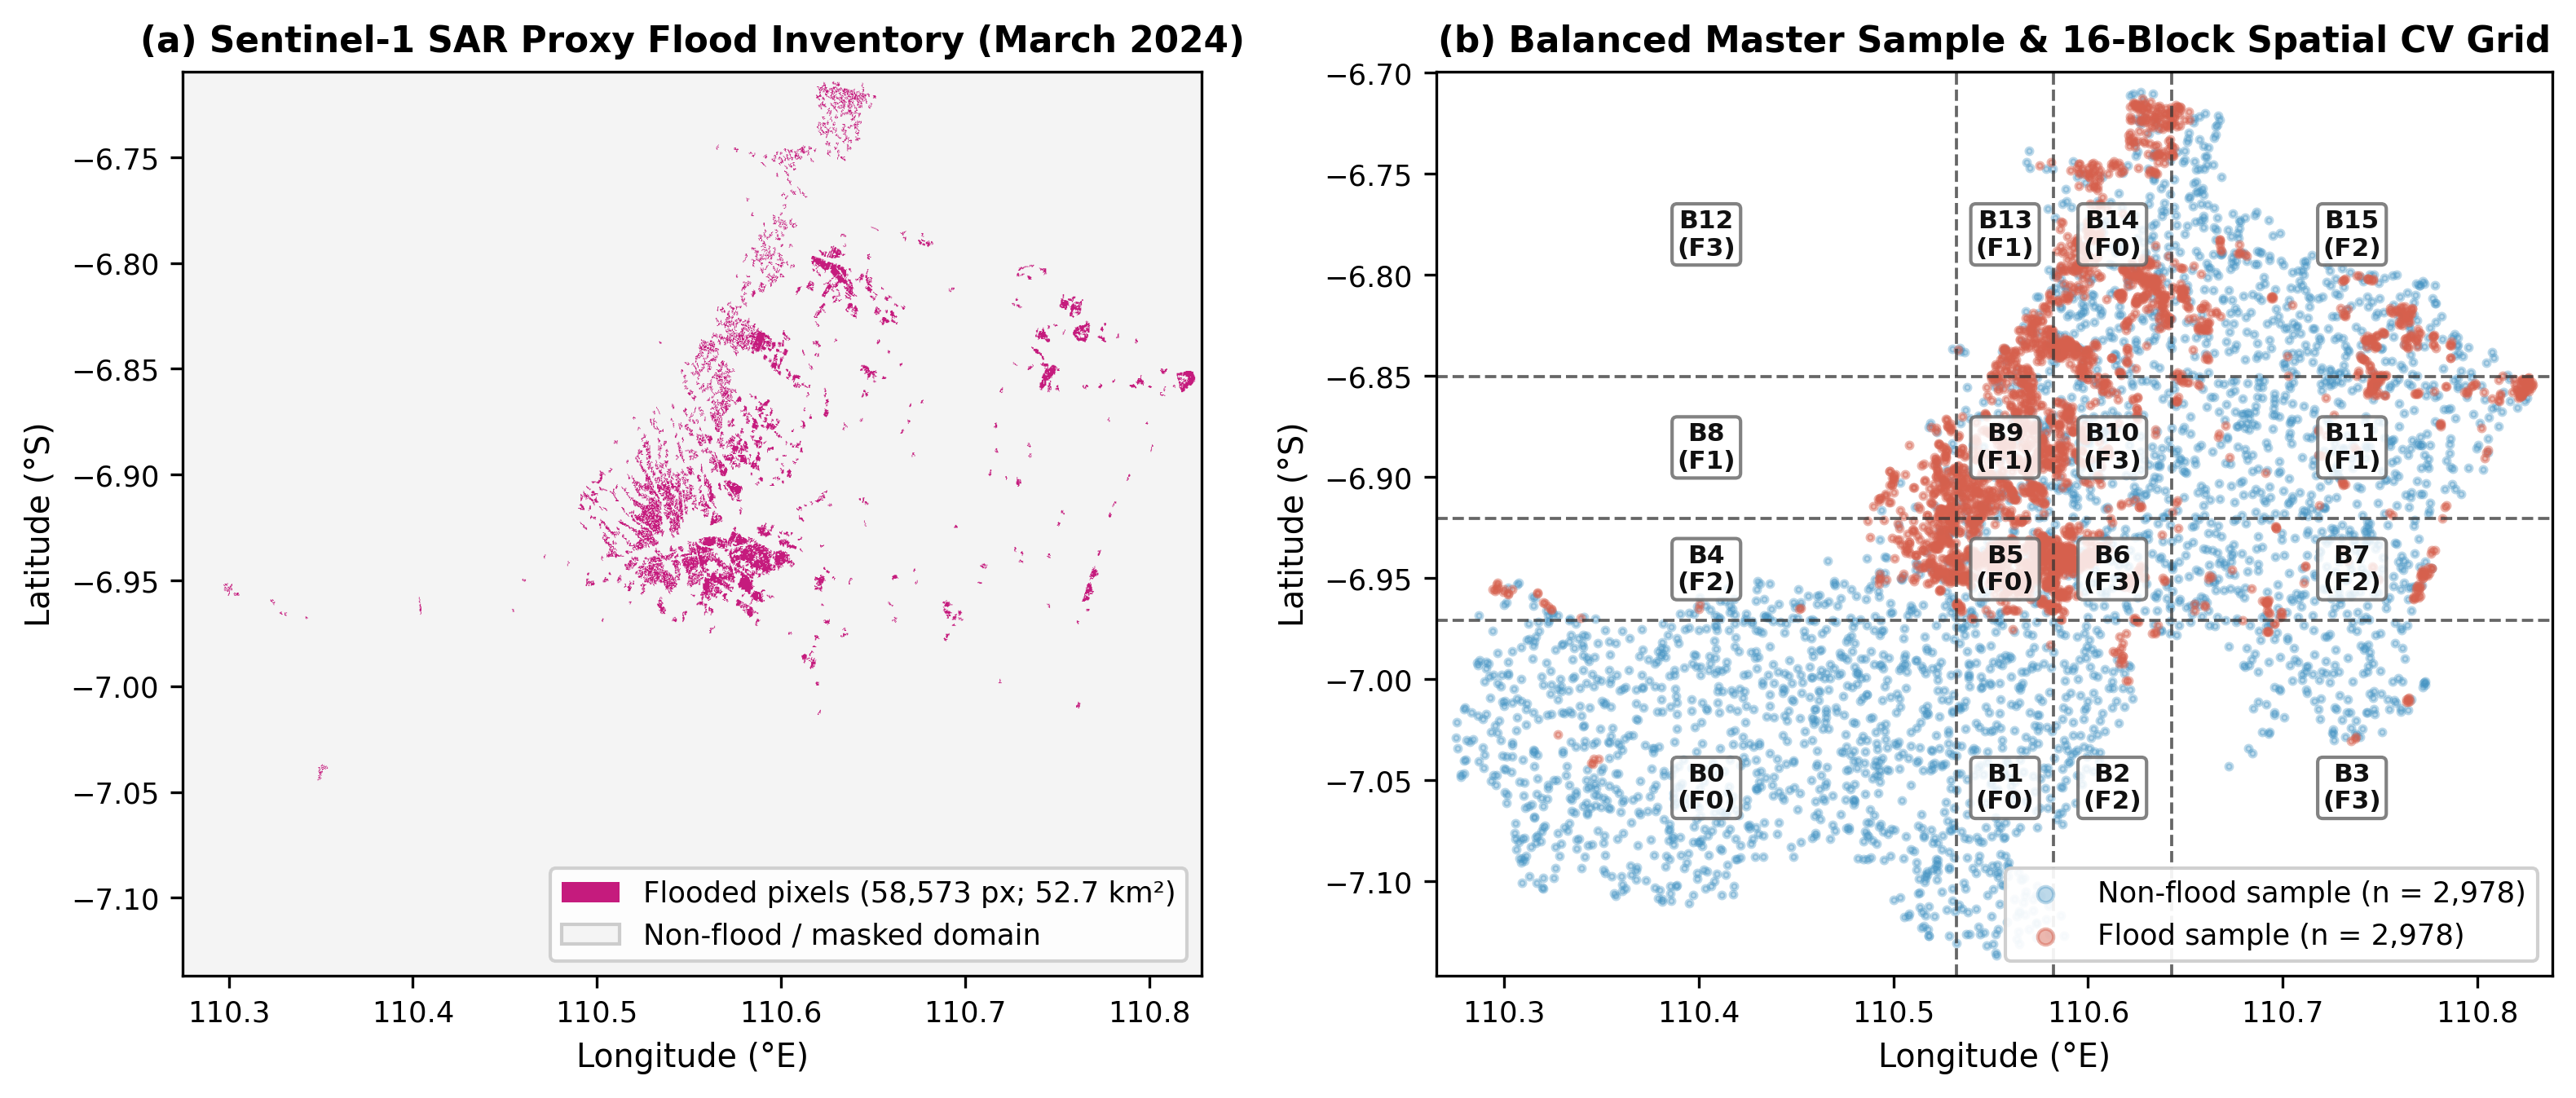
\includegraphics[width=0.94\textwidth]{figures/fig_study_area_samples.png}
\caption{Wilayah kajian dan struktur pengambilan sampel: (a) \textit{flood inventory} proksi Sentinel-1 SAR kejadian Maret 2024 di Semarang--Demak ($58.573$ piksel banjir); (b) sebaran spasial sampel induk berimbang ($n = 5.956$) beserta pembagian 16 blok kuantil koordinat (\texttt{B0}--\texttt{B15}) dan penugasan 4-\textit{fold} validasi silang spasial (\texttt{F0}--\texttt{F3}).}
\label{fig:study-area-id}
\end{figure}

Audit diagnostik mengungkap koreksi metodologis penting pada tahap pengambilan sampel kelas non-banjir. Pita \texttt{occurrence} JRC Global Surface Water bersifat jarang (\textit{sparse}) dan hanya memiliki nilai valid pada $187.777$ piksel ($12{,}78\%$ wilayah kajian). Apabila penyaringan air permanen dilakukan langsung dengan \texttt{permanent\_water.Not()} tanpa \texttt{unmask(0)}, seluruh piksel daratan tanpa riwayat air ikut ter-masking sehingga kandidat sampel non-banjir menyempit ke sabuk sekitar perairan seluas $123.616$ piksel ($8{,}76\%$ dari populasi non-banjir, dengan rata-rata elevasi sampel hanya $4{,}15\text{ m}$ berbanding rata-rata AOI $42{,}7\text{ m}$). Dengan menerapkan \texttt{permanent\_water.unmask(0)} sebelum negasi, kandidat sampel non-banjir pulih mencakup $1.382.033$ piksel ($97{,}95\%$ populasi non-banjir se-AOI). Dari domain yang telah dikoreksi ini, penyampelan terstratifikasi dan penyaringan data lengkap menghasilkan sampel induk berimbang sebanyak $n = 5.956$ titik ($2.978$ banjir dan $2.978$ non-banjir; Gambar~\ref{fig:study-area-id}b). Perlu ditegaskan bahwa Kelas 1 merepresentasikan piksel yang terdeteksi tergenang oleh pipeline proksi SAR (di dalam dukungan spasial JRC $12{,}78\%$ AOI), sedangkan Kelas 0 (``non-banjir'') merepresentasikan piksel yang tidak terdeteksi tergenang oleh pipeline proksi yang sama pada $97{,}95\%$ wilayah non-banjir AOI dan bukan bukti lapangan ketiadaan genangan; prediksi di luar dukungan positif JRC dengan demikian merupakan ekstrapolasi spasial.

\subsection{Ekstraksi Prediktor Turunan DEM dan Prediktor Non-DEM}\label{subsec:prediktor-id}

Dari setiap produk elevasi perlakuan $d \in \{\text{srtm}, \text{glo30}, \text{aw3d30}\}$, diekstraksi lima fitur topografi menggunakan prosedur \texttt{ee.Terrain} yang identik:
\begin{equation}
\mathbf{x}_{\text{DEM}}^{(d)} = \Bigl(\text{elevation}_d,\; \text{slope}_d,\; \sin(\alpha_d),\; \cos(\alpha_d),\; \mathbb{I}(\text{slope}_d > 0)\Bigr),
\label{eq:dem-features-id}
\end{equation}
di mana arah lereng $\alpha_d \in [0^\circ, 360^\circ)$ didekomposisi menjadi komponen sinus dan kosinus (diisi nilai netral $0$ pada piksel datar $\text{slope}_d = 0^\circ$) disertai indikator biner $\text{aspect\_valid}_d = \mathbb{I}(\text{slope}_d > 0)$ guna mengatasi diskontinuitas sudut melingkar $0^\circ/360^\circ$. Sembilan belas prediktor non-DEM dipertahankan identik mengikuti studi acuan \cite{hakim2026}, terdiri atas 4 variabel MERIT Hydro (\texttt{hand}, \texttt{upa\_log}, \texttt{river\_width}, \texttt{dist\_river}) \cite{yamazaki2019}, jarak ke air permanen JRC (\texttt{dist\_perm\_water}) \cite{pekel2016}, curah hujan antecedent 7 dan 30 hari CHIRPS (\texttt{rain\_7d}, \texttt{rain\_30d}) \cite{funk2015}, 4 indeks spektral Sentinel-2 periode kering Juni--Oktober 2023 (\texttt{ndvi}, \texttt{ndwi}, \texttt{mndwi}, \texttt{ndbi}) \cite{saha2021}, serta 8 variabel \textit{dummy} tutupan lahan ESA WorldCover (\texttt{lc\_10}, \texttt{lc\_30}, \texttt{lc\_40}, \texttt{lc\_50}, \texttt{lc\_60}, \texttt{lc\_80}, \texttt{lc\_90}, \texttt{lc\_95}, melalui \textit{one-hot encoding} tanpa membuang kategori acuan (\texttt{drop\_first=False}); karena kelas semak belukar \texttt{lc\_20} tidak muncul pada sampel utama (\texttt{seed=42}) dan \texttt{seed=99}, terbentuk 8 variabel \textit{dummy} ($5 + 11 + 8 = 24$ input), sedangkan pada \textit{seed} 100, 2024, dan 7 terbentuk 9 variabel \textit{dummy} atau 25 input) \cite{zanaga2021}. Berbeda dengan pipeline evaluasi \texttt{scikit-learn} (24/25 input), pemetaan probabilitas spasial di GEE menggunakan \texttt{smileRandomForest} (300 pohon) yang dilatih pada seluruh sampel induk ($n=5.956$) dengan 17 input (5 DEM + 11 kontinu non-DEM + 1 band kategorikal \texttt{landcover}).

\subsection{Evaluasi Model, Validasi Spasial, dan Analisis Sensitivitas}\label{subsec:evaluasi-id}

Evaluasi kinerja dilakukan pertama kali pada pembagian acak terstratifikasi 75:25 ($n_{\text{latih}}=4.467$, $n_{\text{uji}}=1.489$; \textit{seed} = 42) menggunakan Random Forest \texttt{scikit-learn} (400 pohon) dengan metrik ROC-AUC, akurasi, presisi, \textit{recall}, dan F1-\textit{score} pada ambang baku $t=0{,}50$ serta ambang indeks Youden $t^*$ \cite{youden1950}. Untuk mengendalikan efek autokorelasi spasial \cite{roberts2017,ploton2020}, diterapkan tiga pengujian ketahanan: (1) validasi silang spasial 4-\textit{fold} pada 16 blok kuantil bujur dan lintang (Gambar~\ref{fig:study-area-id}b); (2) \textit{block bootstrap} berpasangan 1.000 iterasi pada 16 blok spasial dibandingkan dengan \textit{bootstrap} tingkat piksel; serta (3) replikasi menyeluruh dari tahap penyampelan GEE hingga evaluasi lintas lima nilai \textit{seed} ($\{42, 100, 2024, 7, 99\}$). Pada tingkat spasial, peta probabilitas dari GEE \texttt{smileRandomForest} (300 pohon) dikelompokkan ke dalam lima kelas kerawanan berinterval seragam ($0{,}2; 0{,}4; 0{,}6; 0{,}8$) untuk menghitung rerata selisih probabilitas absolut $\overline{|\Delta p|}$, tingkat kesesuaian kelas (\textit{spatial agreement}), matriks transisi antarkelas, dan stratifikasi sensitivitas per kelas tutupan lahan ESA WorldCover. Selain itu, autokorelasi spasial pada prediksi dan residual \textit{out-of-fold} ($r_i^{\text{OOF}} = y_i - \hat{p}_i^{\text{OOF}}$) pada $n = 5.956$ titik sampel (bobot KNN terstandardisasi baris $k \in \{5, 8, 12\}$ di UTM 49S, $B = 9.999$ permutasi) serta pada raster probabilitas pasca-masking AOI (ketetanggaan Queen 8-tetangga, $B = 999$ permutasi) diuji menggunakan Global Moran's $I$ \cite{moran1950}.

%==================================
\section{Hasil Empiris}\label{sec:hasil}

\subsection{Karakteristik Parameter Topografi Produk Elevasi Global}\label{subsec:hasil-dem}

Statistik deskriptif pada grid 30 meter (Tabel~\ref{tab:dem-stats-id}) menunjukkan bahwa ketiga produk elevasi merepresentasikan pola bentang lahan makro yang sejalan, tetapi berbeda nyata pada distribusi elevasi median dan kemiringan lereng di dataran rendah pesisir. Rata-rata elevasi se-AOI adalah $40{,}62\text{ m}$ (SRTM), $39{,}06\text{ m}$ (Copernicus GLO-30), dan $41{,}36\text{ m}$ (ALOS AW3D30), dengan selisih (\textit{offset}) vertikal rata-rata terhadap SRTM sebesar $-1{,}56\text{ m}$ pada Copernicus GLO-30 dan $+0{,}39\text{ m}$ pada ALOS AW3D30. Namun, median elevasi AOI pada Copernicus GLO-30 ($4{,}94\text{ m}$) jauh lebih rendah dibandingkan SRTM ($8{,}50\text{ m}$) dan ALOS AW3D30 ($8{,}53\text{ m}$).

\begin{table}[!htbp]
\small
\centering
\caption{Statistik deskriptif elevasi (m) dan kemiringan lereng ($^\circ$) pada seluruh grid AOI Semarang--Demak ($N = 1.469.555$ piksel) serta pada titik sampel banjir ($n=2.978$) dan non-banjir ($n=2.978$).}
\label{tab:dem-stats-id}
\begin{adjustbox}{max width=\textwidth}
\begin{tabular}{ll rrrrrrr rr rr}
\toprule
& & \multicolumn{7}{c}{\textbf{Distribusi Grid Seluruh AOI ($N = 1.469.555$ piksel)}} & \multicolumn{2}{c}{\textbf{Sampel Banjir ($n=2.978$)}} & \multicolumn{2}{c}{\textbf{Non-Banjir ($n=2.978$)}} \\
\cmidrule(lr){3-9} \cmidrule(lr){10-11} \cmidrule(lr){12-13}
\textbf{Parameter} & \textbf{Produk DEM} & \textbf{Mean} & \textbf{SD} & $\boldsymbol{p_5}$ & $\boldsymbol{p_{25}}$ & $\boldsymbol{p_{50}}$ & $\boldsymbol{p_{75}}$ & $\boldsymbol{p_{95}}$ & \textbf{Mean} & \textbf{Median} & \textbf{Mean} & \textbf{Median} \\
\midrule
Elevasi (m) & SRTM & 40,62 & 76,09 & 0,60 & 4,53 & 8,50 & 24,60 & 234,51 & 3,25 & 3,00 & 42,67 & 8,00 \\
            & Copernicus GLO-30 & 39,06 & 75,72 & 1,18 & 2,96 & 4,94 & 22,97 & 233,00 & 1,99 & 1,40 & 41,12 & 6,30 \\
            & ALOS AW3D30 & 41,36 & 76,22 & 2,77 & 4,47 & 8,53 & 24,52 & 234,48 & 4,11 & 4,00 & 43,06 & 8,00 \\
\midrule
Slope ($^\circ$) & SRTM & 3,03 & 3,38 & 0,00 & 1,35 & 2,13 & 3,43 & 9,63 & 1,73 & 1,35 & 3,08 & 2,12 \\
                 & Copernicus GLO-30 & 2,46 & 3,99 & 0,14 & 0,36 & 0,87 & 2,87 & 10,62 & 0,39 & 0,28 & 2,59 & 0,93 \\
                 & ALOS AW3D30 & 3,13 & 4,02 & 0,00 & 0,95 & 1,90 & 3,43 & 10,92 & 1,32 & 0,96 & 3,17 & 1,91 \\
\bottomrule
\end{tabular}
\end{adjustbox}
\end{table}

Pada parameter kemiringan lereng (\textit{slope}), Copernicus GLO-30 menghasilkan permukaan dataran rendah yang jauh lebih halus (median AOI $0{,}87^\circ$, rata-rata $2{,}46^\circ$) dibandingkan ALOS AW3D30 (median $1{,}90^\circ$) dan SRTM (median $2{,}13^\circ$). Pada $2.978$ titik sampel banjir (Gambar~\ref{fig:dem-characteristics-id}), genangan terkonsentrasi di dataran rendah pesisir dengan median elevasi $3{,}00\text{ m}$ (SRTM), $1{,}40\text{ m}$ (GLO-30), dan $4{,}00\text{ m}$ (AW3D30), serta median kemiringan lereng masing-masing $1{,}35^\circ$, $0{,}28^\circ$, dan $0{,}96^\circ$. Sebanyak $98{,}99\%$ (SRTM), $99{,}97\%$ (GLO-30), dan $98{,}76\%$ (AW3D30) titik banjir berada di bawah kemiringan $5^\circ$, sedangkan 30 titik banjir ($1{,}01\%$) yang memiliki fitur prediktor \texttt{slope\_srtm} $\ge 5^\circ$ ($5{,}10^\circ\text{--}11{,}48^\circ$) telah terverifikasi melalui diagnostik 4 rute GEE memiliki lereng asli \texttt{EPSG:4326} $<5^\circ$ pada seluruh 30/30 titik ($1{,}32^\circ\text{--}4{,}99^\circ$) saat pembentukan label (\texttt{slope.lt(5)}), dan bergeser menjadi $\ge 5^\circ$ akibat reproyeksi ke grid analisis \texttt{EPSG:32749} (30\,m) sebelum perhitungan lereng prediktor (selisih $0{,}000000^\circ$ terhadap CSV sampel induk).

\begin{figure}[!htbp]
\centering
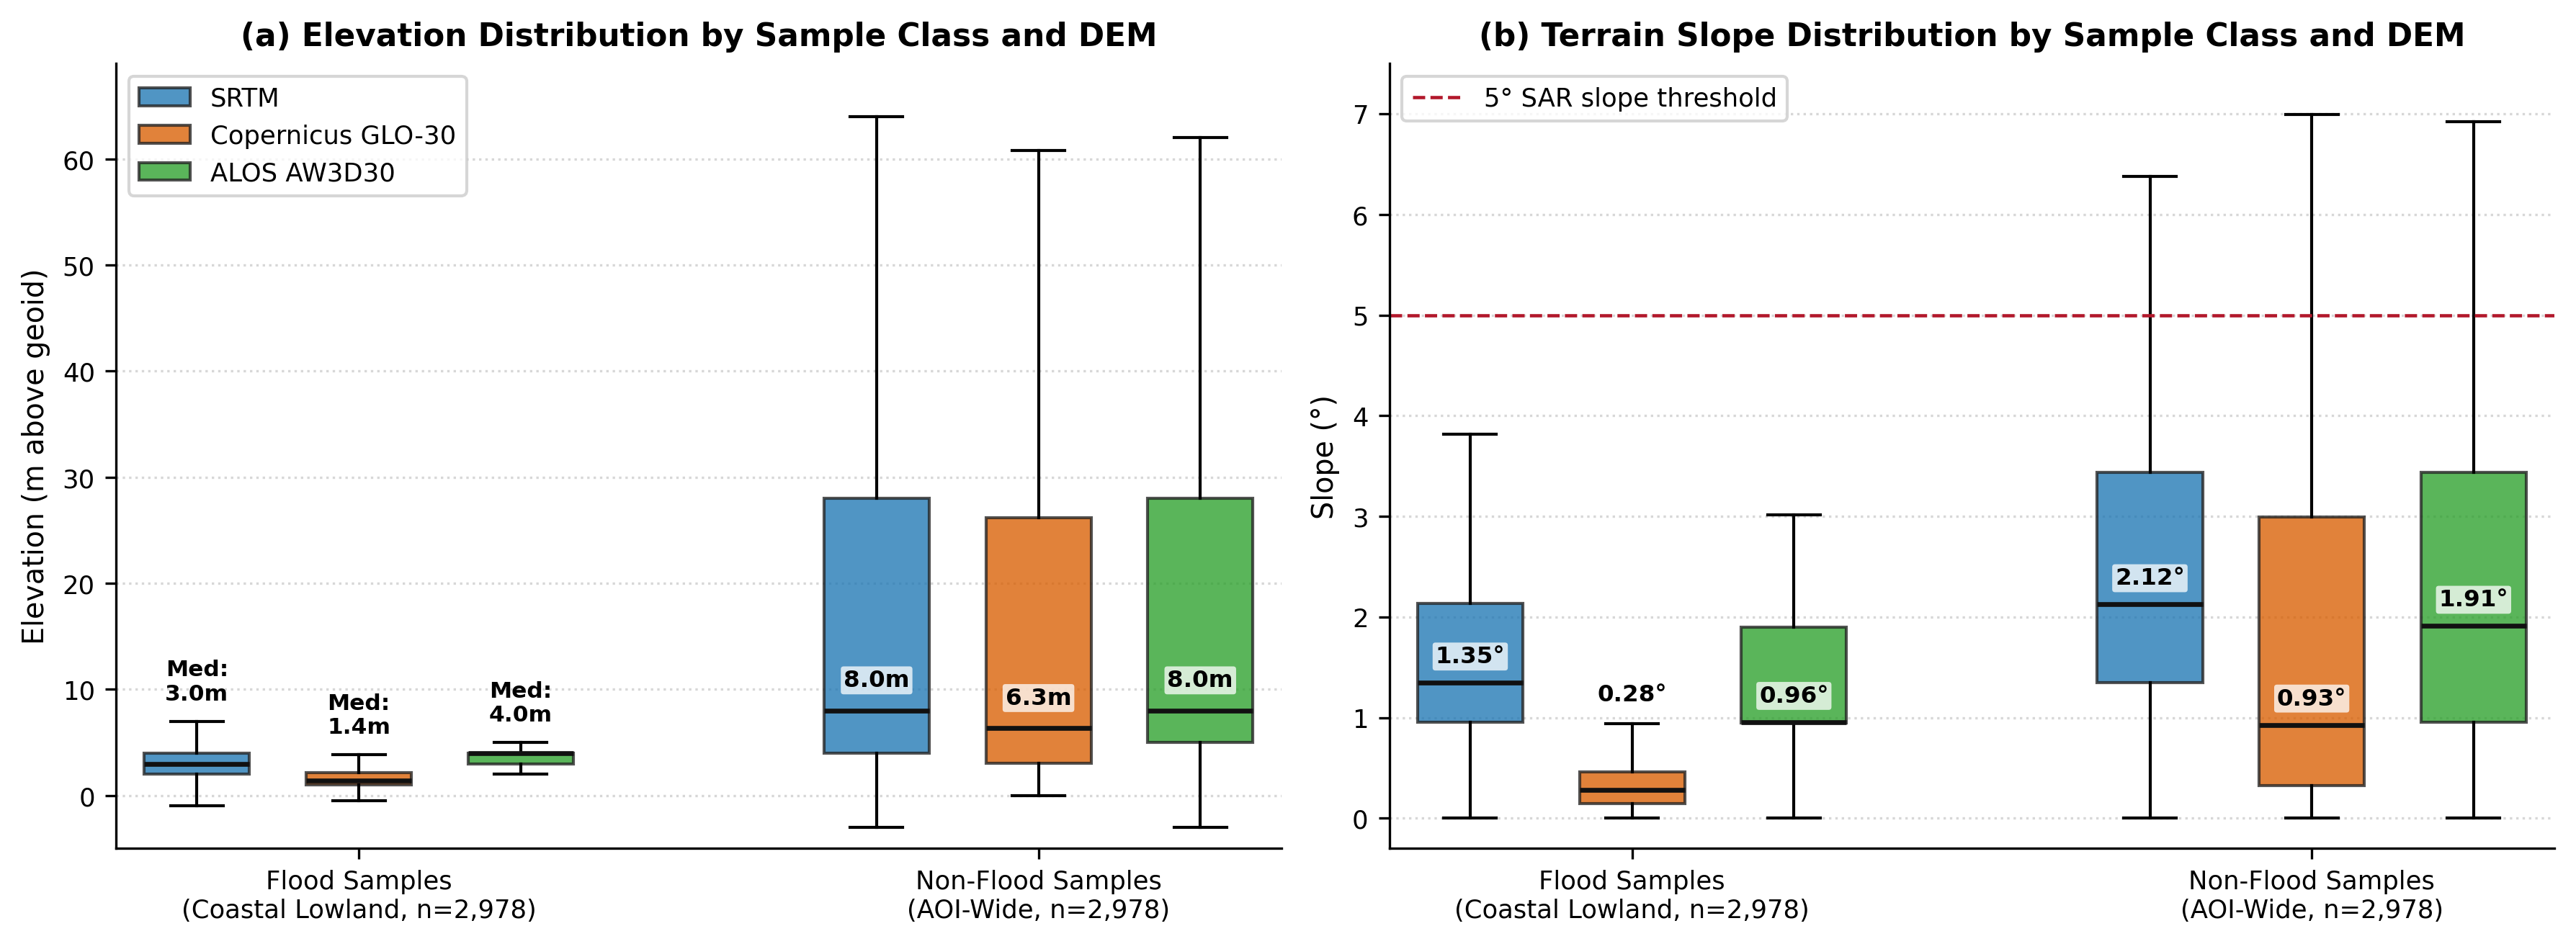
\includegraphics[width=0.94\textwidth]{figures/fig_dem_characteristics.png}
\caption{Distribusi empiris (a) elevasi dan (b) kemiringan lereng pada titik sampel banjir ($n = 2.978$) dan non-banjir ($n = 2.978$) untuk SRTM, Copernicus DEM GLO-30, dan ALOS AW3D30.}
\label{fig:dem-characteristics-id}
\end{figure}

\subsection{Kinerja Prediktif pada Evaluasi Holdout dan Validasi Silang Spasial}\label{subsec:hasil-performa}

Tabel~\ref{tab:holdout-id} merangkum kinerja ketiga konfigurasi DEM pada data uji \textit{holdout} acak terstratifikasi ($n_{\text{uji}}=1.489$; \textit{seed} = 42). Ketiga produk elevasi menghasilkan daya diskriminasi yang tinggi dengan urutan konsisten: Copernicus DEM GLO-30 ($\text{ROC-AUC} = 0{,}9404$) $>$ ALOS AW3D30 ($0{,}9360$) $>$ SRTM ($0{,}9318$). Pada ambang baku $t=0{,}50$, Copernicus GLO-30 mencapai akurasi ($0{,}8899$), presisi ($0{,}8580$), \textit{recall} ($0{,}9341$), dan F1-\textit{score} ($0{,}8945$) tertinggi (Gambar~\ref{fig:roc-id} dan Gambar~\ref{fig:cm-id}).

\begin{table}[!htbp]
\small
\centering
\caption{Metrik evaluasi \textit{holdout} acak terstratifikasi ($n_{\text{uji}} = 1.489$; \textit{seed} = 42) pada ambang baku ($t = 0{,}50$) dan ambang optimal indeks Youden ($t^*$).}
\label{tab:holdout-id}
\begin{adjustbox}{max width=\textwidth}
\begin{tabular}{l c cccc c cccc c}
\toprule
& & \multicolumn{4}{c}{\textbf{Ambang Klasifikasi Baku ($t = 0{,}50$)}} & & \multicolumn{4}{c}{\textbf{Ambang Optimal Indeks Youden ($t^*$)}} & \\
\cmidrule(lr){3-6} \cmidrule(lr){8-11}
\textbf{Konfigurasi DEM} & \textbf{ROC-AUC} & \textbf{Akurasi} & \textbf{Presisi} & \textbf{Recall} & \textbf{F1-Score} & $\boldsymbol{t^*}$ & \textbf{Akurasi} & \textbf{Presisi} & \textbf{Recall} & \textbf{F1-Score} & $\boldsymbol{\Delta}\textbf{AUC vs.\ SRTM}$ \\
\midrule
SRTM & 0,9318 & 0,8744 & 0,8468 & 0,9140 & 0,8791 & 0,5205 & 0,8791 & 0,8588 & 0,9073 & 0,8824 & $0{,}0000$ \\
Copernicus GLO-30 & \textbf{0,9404} & \textbf{0,8899} & \textbf{0,8580} & \textbf{0,9341} & \textbf{0,8945} & 0,4953 & \textbf{0,8912} & 0,8584 & \textbf{0,9368} & \textbf{0,8959} & $+0{,}0086$ \\
ALOS AW3D30 & 0,9360 & 0,8784 & 0,8488 & 0,9207 & 0,8833 & 0,5209 & 0,8805 & 0,8555 & 0,9153 & 0,8844 & $+0{,}0042$ \\
\bottomrule
\end{tabular}
\end{adjustbox}
\end{table}

\begin{figure}[!htbp]
\centering
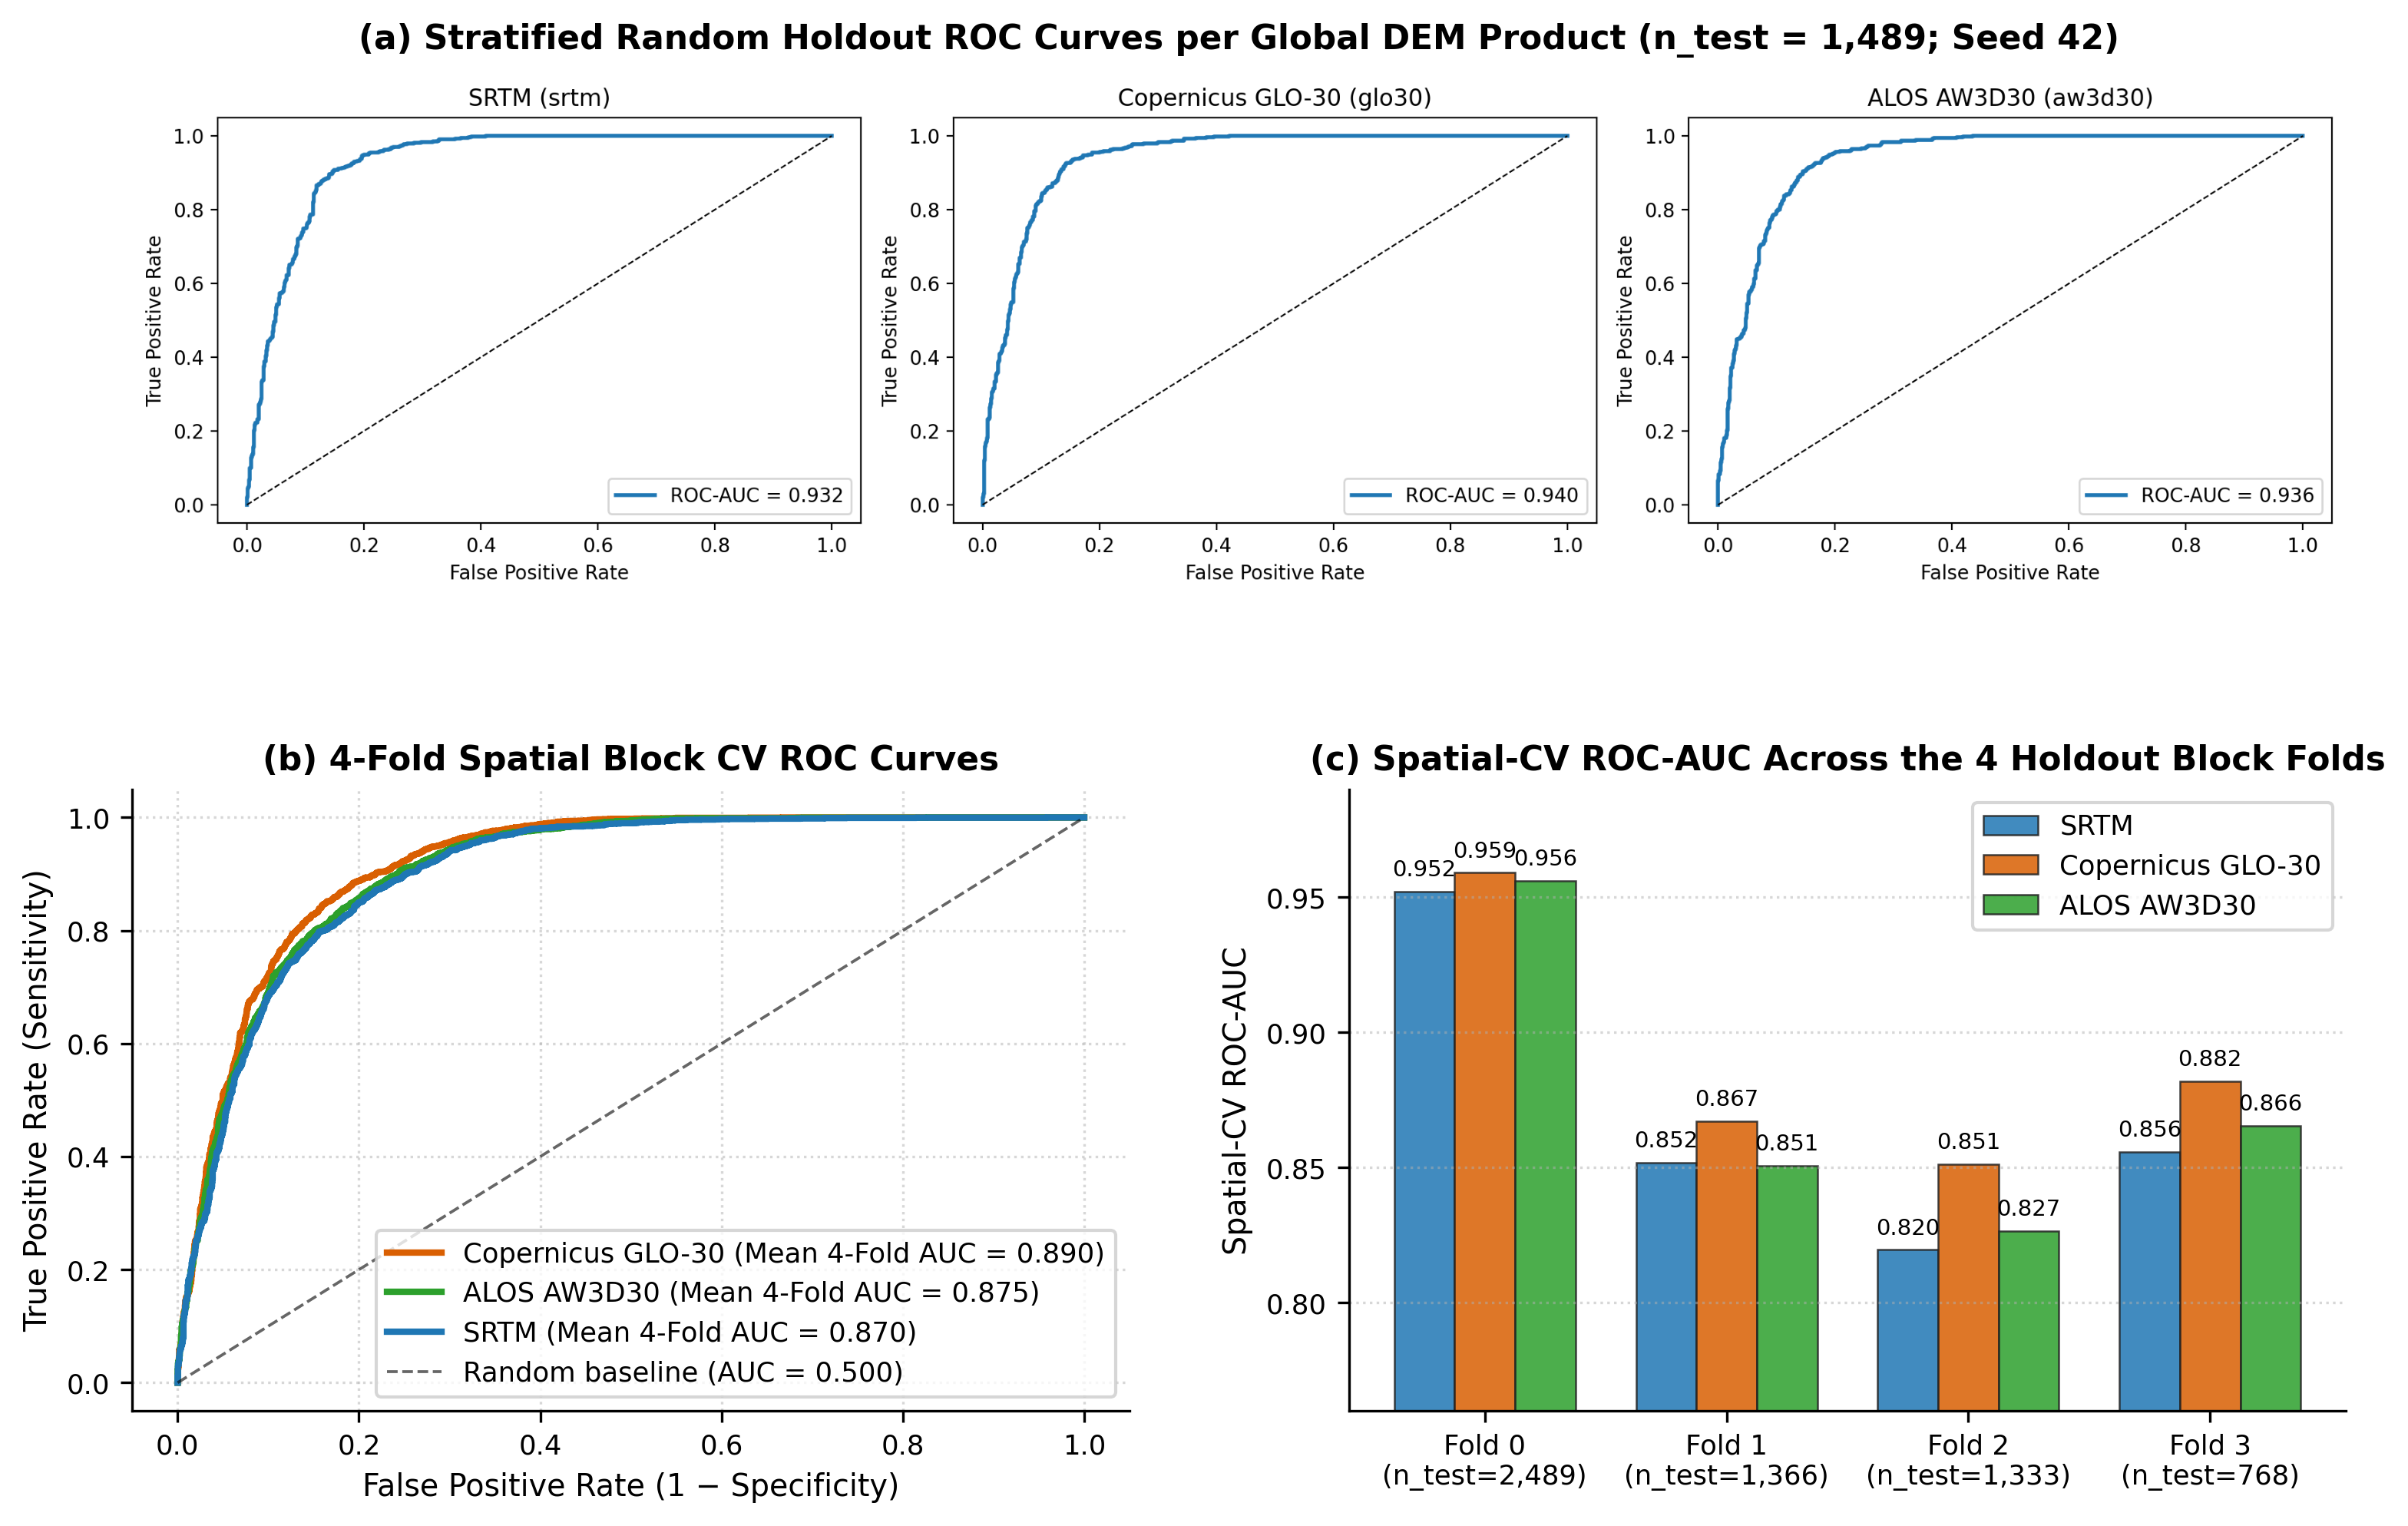
\includegraphics[width=0.94\textwidth]{figures/fig_roc.png}
\caption{Kurva dan metrik ROC lintas skema evaluasi: (a) kurva ROC \textit{holdout} acak terstratifikasi ($n_{\text{uji}} = 1.489$); (b) kurva ROC gabungan validasi silang spasial 4-\textit{fold}; dan (c) perbandingan ROC-AUC per \textit{fold} spasial.}
\label{fig:roc-id}
\end{figure}

\begin{figure}[!htbp]
\centering
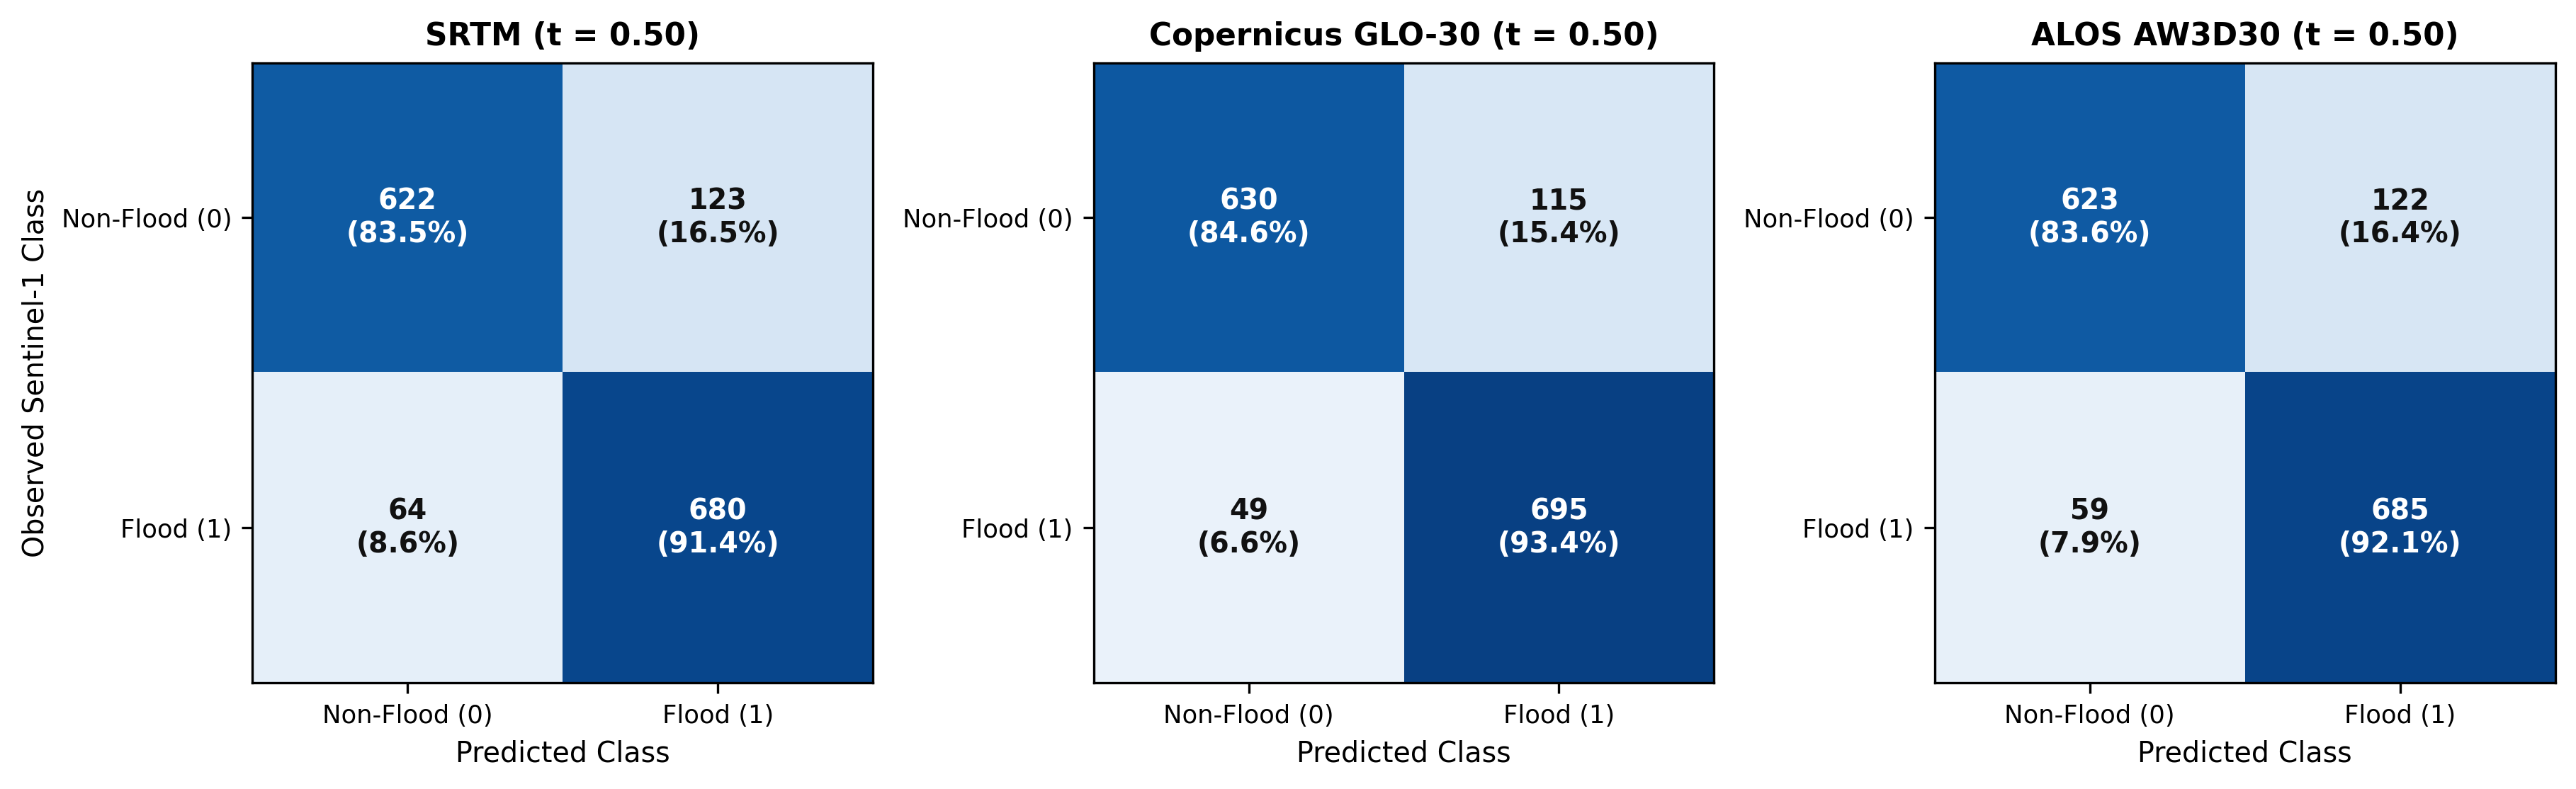
\includegraphics[width=0.94\textwidth]{figures/fig_confusion_matrices.png}
\caption{Matriks konfusi pada data uji \textit{holdout} ($n_{\text{uji}} = 1.489$; ambang $t = 0{,}50$) untuk SRTM, Copernicus DEM GLO-30, dan ALOS AW3D30.}
\label{fig:cm-id}
\end{figure}

Pada skema validasi silang spasial 4-\textit{fold} lintas 16 blok kuantil (Tabel~\ref{tab:spatial-cv-id}), rata-rata ROC-AUC berbasis probabilitas tercatat sebesar $0{,}8699$ (SRTM), $0{,}8747$ (ALOS AW3D30), dan $0{,}8899$ (Copernicus GLO-30), dengan keunggulan Copernicus GLO-30 bertahan konsisten di seluruh empat \textit{fold} spasial.

\begin{table}[!htbp]
\small
\centering
\caption{Hasil validasi silang spasial 4-\textit{fold} lintas 16 blok kuantil koordinat (\textit{seed} = 42).}
\label{tab:spatial-cv-id}
\begin{adjustbox}{max width=\textwidth}
\begin{tabular}{c c c c l cccccc}
\toprule
\textbf{Fold} & \textbf{Blok Uji} & $\boldsymbol{n_{\text{latih}}}$ & $\boldsymbol{n_{\text{uji}}}$ & \textbf{Konfigurasi DEM} & $\textbf{AUC}_{\textbf{prob}}$ & $\textbf{AUC}_{\textbf{biner}}$ & \textbf{Akurasi} & \textbf{Presisi} & \textbf{Recall} & \textbf{F1-Score} \\
\midrule
0 & $\{0, 1, 5, 14\}$ & 3.467 & 2.489 & SRTM & 0,9521 & 0,8667 & 0,8734 & 0,8755 & 0,8203 & 0,8470 \\
  & & & & Copernicus GLO-30 & \textbf{0,9591} & \textbf{0,9047} & \textbf{0,9052} & 0,8797 & \textbf{0,9012} & \textbf{0,8903} \\
  & & & & ALOS AW3D30 & 0,9562 & 0,8870 & 0,8911 & \textbf{0,8830} & 0,8589 & 0,8708 \\
\midrule
1 & $\{8, 9, 11, 13\}$ & 4.590 & 1.366 & SRTM & 0,8519 & 0,7890 & 0,8302 & 0,8573 & \textbf{0,9014} & 0,8788 \\
  & & & & Copernicus GLO-30 & \textbf{0,8673} & \textbf{0,8119} & \textbf{0,8360} & \textbf{0,8816} & 0,8778 & \textbf{0,8797} \\
  & & & & ALOS AW3D30 & 0,8508 & 0,7891 & 0,8184 & 0,8655 & 0,8692 & 0,8674 \\
\midrule
2 & $\{2, 4, 7, 15\}$ & 4.623 & 1.333 & SRTM & 0,8197 & 0,7279 & 0,7374 & \textbf{0,6939} & 0,6691 & 0,6812 \\
  & & & & Copernicus GLO-30 & \textbf{0,8514} & \textbf{0,7523} & \textbf{0,7539} & 0,6928 & \textbf{0,7424} & \textbf{0,7168} \\
  & & & & ALOS AW3D30 & 0,8265 & 0,7177 & 0,7269 & 0,6796 & 0,6601 & 0,6697 \\
\midrule
3 & $\{3, 6, 10, 12\}$ & 5.188 & 768 & SRTM & 0,8559 & 0,7694 & 0,7669 & 0,8161 & 0,7447 & 0,7787 \\
  & & & & Copernicus GLO-30 & \textbf{0,8820} & \textbf{0,7991} & \textbf{0,8008} & \textbf{0,8214} & \textbf{0,8156} & \textbf{0,8185} \\
  & & & & ALOS AW3D30 & 0,8655 & 0,7806 & 0,7812 & 0,8102 & 0,7872 & 0,7986 \\
\midrule
\multicolumn{4}{l}{\textbf{Rata-Rata Lintas 4 Fold Spasial}} & SRTM & 0,8699 & 0,7883 & 0,8020 & 0,8107 & 0,7839 & 0,7964 \\
\multicolumn{4}{l}{} & Copernicus GLO-30 & \textbf{0,8899} & \textbf{0,8170} & \textbf{0,8240} & \textbf{0,8189} & \textbf{0,8343} & \textbf{0,8263} \\
\multicolumn{4}{l}{} & ALOS AW3D30 & 0,8747 & 0,7936 & 0,8044 & 0,8096 & 0,7939 & 0,8016 \\
\bottomrule
\end{tabular}
\end{adjustbox}
\end{table}

\subsection{Inferensi Block Bootstrap dan Ketahanan Multi-Seed}\label{subsec:bootstrap-id}

Pengujian \textit{block bootstrap} 1.000 iterasi pada 16 blok spasial (Tabel~\ref{tab:bootstrap-id} dan Gambar~\ref{fig:bootstrap-id}a) menunjukkan bahwa selisih ROC-AUC antara SRTM dan Copernicus GLO-30 ($\Delta\text{AUC} = -0{,}0155$, CI 95\% $[-0{,}0250; -0{,}0072]$) serta antara Copernicus GLO-30 dan ALOS AW3D30 ($\Delta\text{AUC} = +0{,}0108$, CI 95\% $[+0{,}0041; +0{,}0198]$) tidak memuat nilai nol, sehingga keunggulan Copernicus GLO-30 konsisten secara statistik pada tingkat blok. Sebaliknya, selisih antara SRTM dan ALOS AW3D30 ($\Delta\text{AUC} = -0{,}0047$, CI 95\% $[-0{,}0096; +0{,}0013]$) memuat nilai nol pada \textit{block bootstrap}, sehingga peringkat keduanya belum dapat dipisahkan secara tegas. Replikasi menyeluruh pada lima nilai \textit{seed} (Tabel~\ref{tab:multiseed-id} dan Gambar~\ref{fig:bootstrap-id}b) mengonfirmasi bahwa peringkat Copernicus GLO-30 $>$ ALOS AW3D30 $>$ SRTM bertahan stabil lintas seluruh \textit{seed}.

\begin{table}[!htbp]
\small
\centering
\caption{Perbandingan $\Delta\text{AUC}$ berpasangan pada \textit{block bootstrap} 16 blok vs.\ \textit{bootstrap} piksel, serta kestabilan lintas lima \textit{seed} ($\{7, 42, 99, 100, 2024\}$).}
\label{tab:bootstrap-id}
\begin{adjustbox}{max width=\textwidth}
\begin{tabular}{l rrrr rrr rr}
\toprule
& \multicolumn{4}{c}{\textbf{Block Bootstrap 16 Blok ($B=1.000$)}} & \multicolumn{3}{c}{\textbf{Bootstrap Piksel ($B=1.000$)}} & \multicolumn{2}{c}{\textbf{Replikasi 5-Seed ($\text{Mean} \pm \text{SD}$)}} \\
\cmidrule(lr){2-5} \cmidrule(lr){6-8} \cmidrule(lr){9-10}
\textbf{Pasangan Produk DEM} & $\boldsymbol{\Delta}\textbf{AUC}$ & \textbf{SD} & \textbf{CI 95\%} & \textbf{Tanpa 0?} & $\boldsymbol{\Delta}\textbf{AUC}$ & \textbf{CI 95\%} & \textbf{Tanpa 0?} & \textbf{Holdout $\boldsymbol{\Delta}$AUC} & \textbf{Spatial-CV $\boldsymbol{\Delta}$AUC} \\
\midrule
SRTM minus GLO-30 & $-0{,}0155$ & 0,0047 & $[-0{,}0250; -0{,}0072]$ & Ya & $-0{,}0141$ & $[-0{,}0173; -0{,}0109]$ & Ya & $-0{,}0082 \pm 0{,}0048$ & $-0{,}0200 \pm 0{,}0039$ \\
SRTM minus AW3D30 & $-0{,}0047$ & 0,0028 & $[-0{,}0096; +0{,}0013]$ & Tidak (Marginal) & $-0{,}0048$ & $[-0{,}0074; -0{,}0023]$ & Ya (Semu) & $-0{,}0012 \pm 0{,}0021$ & $-0{,}0079 \pm 0{,}0034$ \\
GLO-30 minus AW3D30 & $+0{,}0108$ & 0,0042 & $[+0{,}0041; +0{,}0198]$ & Ya & $+0{,}0094$ & $[+0{,}0063; +0{,}0124]$ & Ya & $+0{,}0070 \pm 0{,}0027$ & $+0{,}0121 \pm 0{,}0055$ \\
\bottomrule
\end{tabular}
\end{adjustbox}
\end{table}

\begin{figure}[!htbp]
\centering
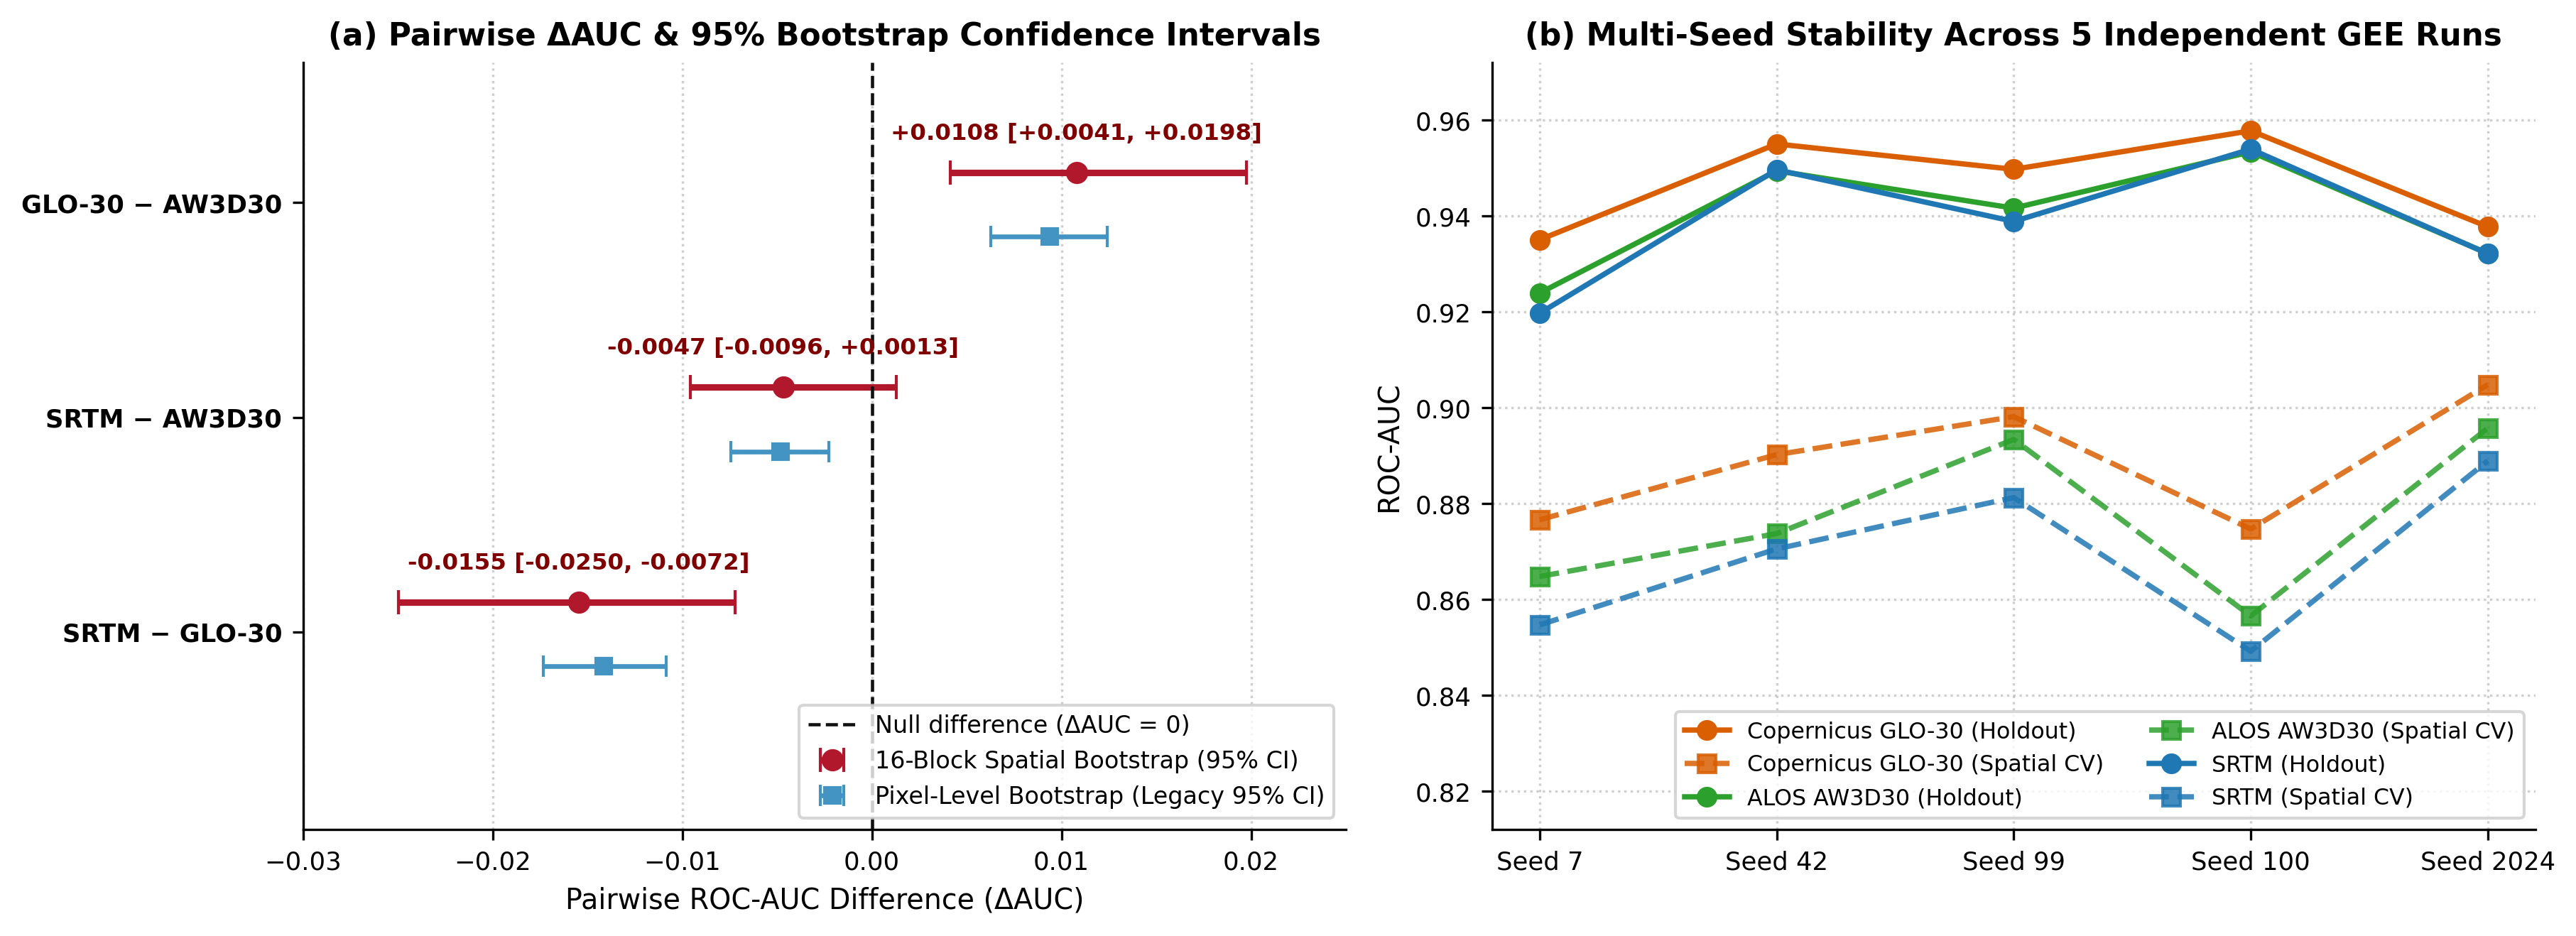
\includegraphics[width=0.94\textwidth]{figures/fig_bootstrap_multiseed.png}
\caption{Inferensi statistik dan ketahanan multi-\textit{seed}: (a) selang kepercayaan 95\% $\Delta\text{AUC}$ pada \textit{block bootstrap} 16 blok vs.\ \textit{bootstrap} piksel; (b) stabilitas ROC-AUC lintas lima \textit{seed} independen ($7, 42, 99, 100, 2024$).}
\label{fig:bootstrap-id}
\end{figure}

\begin{table}[!htbp]
\small
\centering
\caption{Ringkasan evaluasi ketahanan multi-\textit{seed} lintas lima eksekusi independen di Google Earth Engine.}
\label{tab:multiseed-id}
\begin{adjustbox}{max width=\textwidth}
\begin{tabular}{l ccccc c c}
\toprule
& \multicolumn{5}{c}{\textbf{ROC-AUC Validasi Spasial per Seed (ROC-AUC Holdout dalam Kurung)}} & \multicolumn{2}{c}{\textbf{Rata-Rata $\pm$ SD (5 Seed)}} \\
\cmidrule(lr){2-6} \cmidrule(lr){7-8}
\textbf{Konfigurasi DEM} & \textbf{Seed 7} & \textbf{Seed 42} & \textbf{Seed 99} & \textbf{Seed 100} & \textbf{Seed 2024} & \textbf{Holdout AUC} & \textbf{Spatial-CV AUC} \\
\midrule
SRTM & 0,8547 (0,9197) & 0,8706 (0,9497) & 0,8813 (0,9389) & 0,8492 (0,9540) & 0,8890 (0,9322) & $0{,}9389 \pm 0{,}0138$ & $0{,}8689 \pm 0{,}0169$ \\
Copernicus GLO-30 & \textbf{0,8767} (\textbf{0,9351}) & \textbf{0,8902} (\textbf{0,9551}) & \textbf{0,8982} (\textbf{0,9498}) & \textbf{0,8747} (\textbf{0,9578}) & \textbf{0,9049} (\textbf{0,9378}) & $\mathbf{0{,}9471 \pm 0{,}0102}$ & $\mathbf{0{,}8889 \pm 0{,}0132}$ \\
ALOS AW3D30 & 0,8648 (0,9240) & 0,8738 (0,9495) & 0,8934 (0,9417) & 0,8566 (0,9534) & 0,8958 (0,9322) & $0{,}9402 \pm 0{,}0121$ & $0{,}8769 \pm 0{,}0173$ \\
\bottomrule
\end{tabular}
\end{adjustbox}
\end{table}

\subsection{Sensitivitas Spasial, Stratifikasi WorldCover, dan Diagnostik Moran's $I$}\label{subsec:spasial-worldcover-id}

Perbandingan spasial pasca-masking AOI ($1.444.085$ piksel valid pada SRTM/GLO-30 dan $1.429.582$ piksel valid pada AW3D30; Tabel~\ref{tab:sensitivitas-id} dan Gambar~\ref{fig:prob-maps-id}--\ref{fig:spatial-id}) memperlihatkan bahwa kesesuaian 5 kelas tertinggi terjadi antara SRTM dan ALOS AW3D30 ($84{,}27\%$, $\overline{|\Delta p|} = 0{,}0371$), diikuti pasangan GLO-30 dan AW3D30 ($81{,}52\%$, $\overline{|\Delta p|} = 0{,}0483$), serta pasangan SRTM dan GLO-30 ($79{,}36\%$, $\overline{|\Delta p|} = 0{,}0556$). Pasca-masking AOI, Copernicus DEM GLO-30 memperluas Kelas 1 (Sangat Rendah) menjadi $822{,}64\text{ km}^2$ (vs.\ $756{,}71\text{ km}^2$ pada SRTM) dan Kelas 5 (Sangat Tinggi) menjadi $109{,}63\text{ km}^2$ (vs.\ $100{,}58\text{ km}^2$ pada SRTM, $+9{,}0\%$), sedangkan ALOS AW3D30 menyusutkan Kelas 5 menjadi $95{,}93\text{ km}^2$ ($-4{,}6\%$ terhadap SRTM).

\begin{figure}[!htbp]
\centering
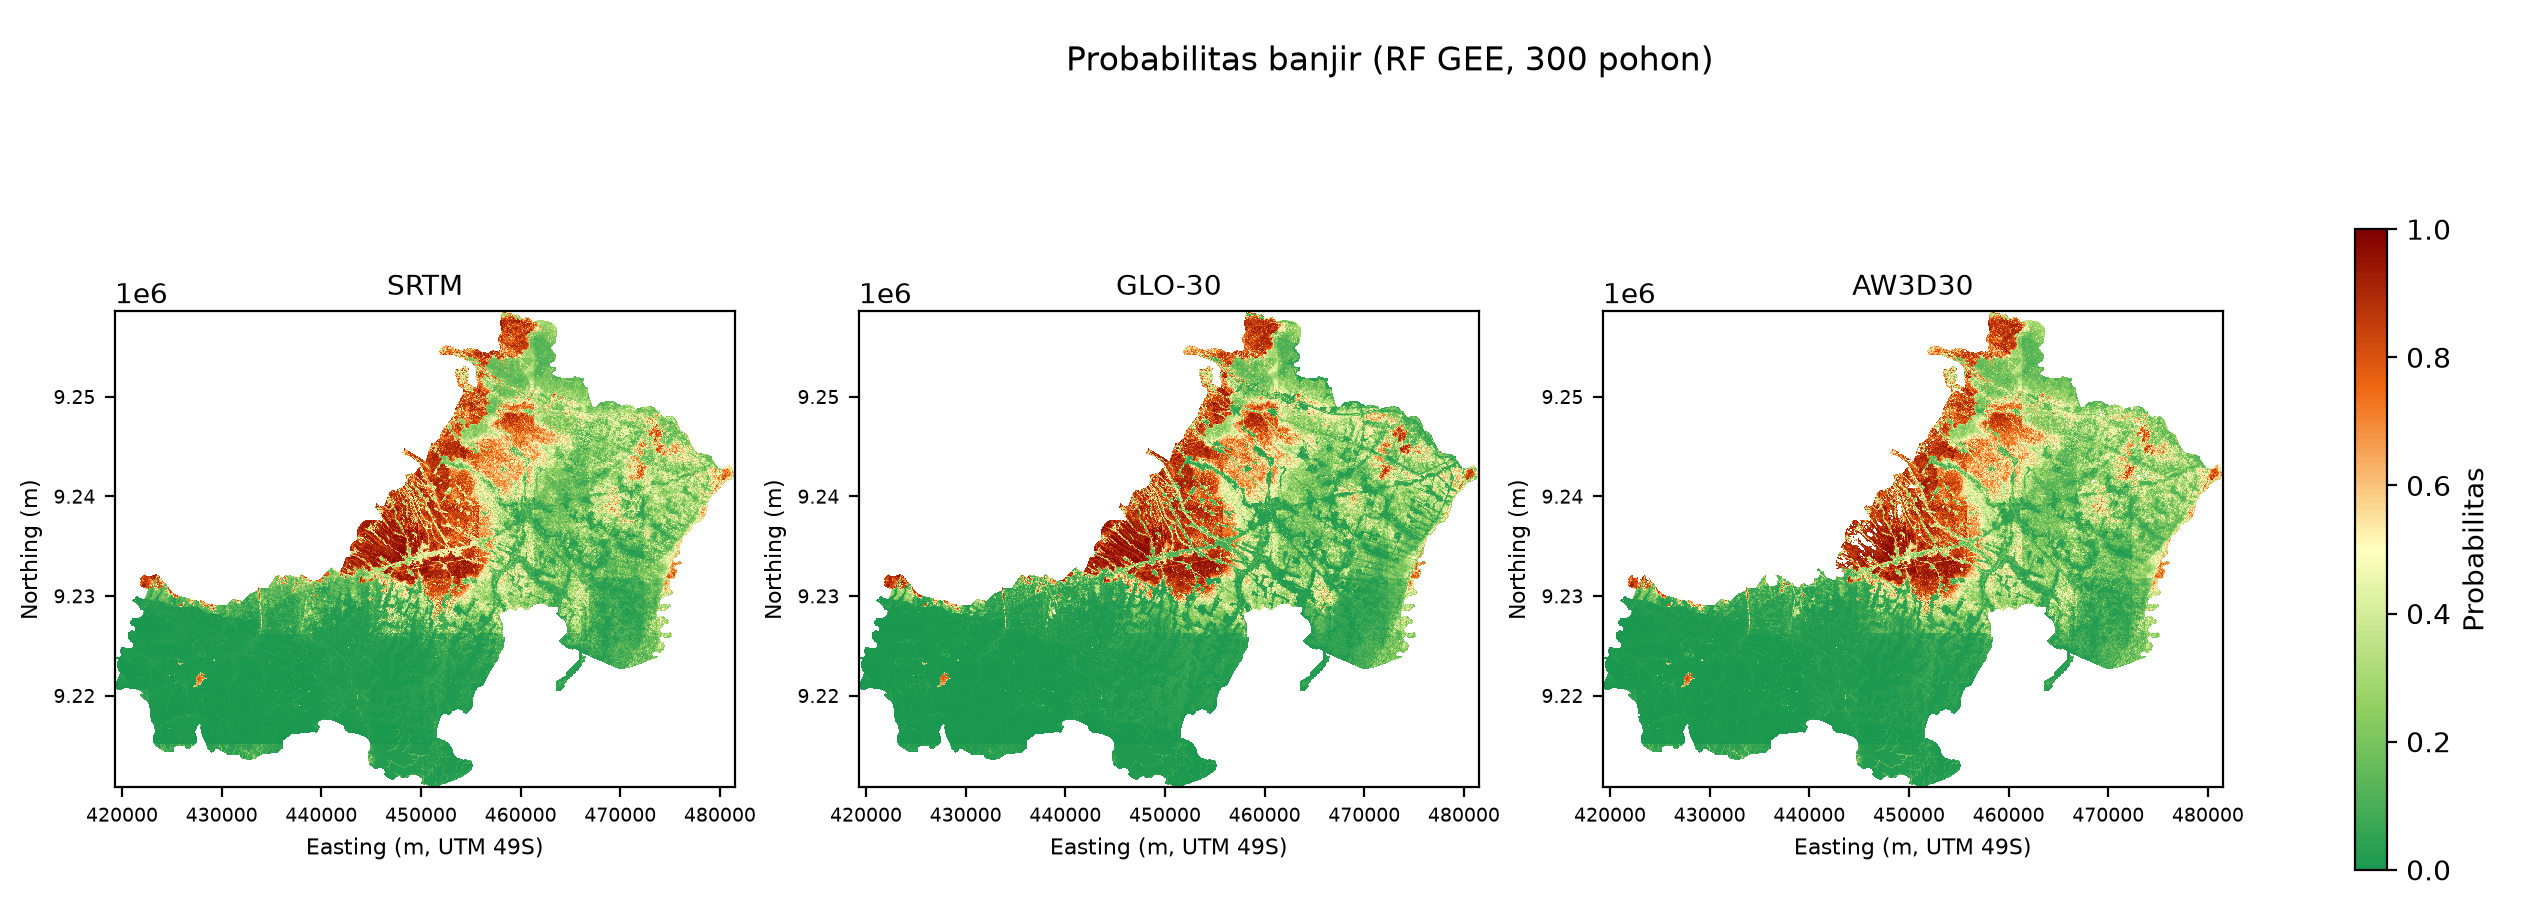
\includegraphics[width=0.96\textwidth]{figures/fig_prob_maps.png}
\caption{Peta probabilitas kerawanan banjir pasca-masking AOI ($p_d(x)$) di koridor pesisir Semarang--Demak dari GEE \texttt{smileRandomForest} (300 pohon) untuk SRTM, Copernicus DEM GLO-30, dan ALOS AW3D30.}
\label{fig:prob-maps-id}
\end{figure}

\begin{table}[!htbp]
\small
\centering
\caption{Distribusi luas kelas kerawanan banjir ($\text{km}^2$ dan \%) serta ringkasan sensitivitas spasial berpasangan pasca-masking AOI di wilayah Semarang--Demak.}
\label{tab:sensitivitas-id}
\begin{adjustbox}{max width=\textwidth}
\begin{tabular}{l rrr rrr l cc}
\toprule
& \multicolumn{3}{c}{\textbf{Luas Area Terpetakan ($\text{km}^2$)}} & \multicolumn{3}{c}{\textbf{Proporsi Wilayah (\%)}} & & \multicolumn{2}{c}{\textbf{Sensitivitas Spasial Berpasangan}} \\
\cmidrule(lr){2-4} \cmidrule(lr){5-7} \cmidrule(lr){9-10}
\textbf{Kelas Kerawanan (Interval Probabilitas)} & \textbf{SRTM} & \textbf{GLO-30} & \textbf{AW3D30} & \textbf{SRTM} & \textbf{GLO-30} & \textbf{AW3D30} & \textbf{Pasangan DEM} & $\boldsymbol{\overline{|\Delta p|}}$ & \textbf{Kesesuaian Kelas (\%)} \\
\midrule
Kelas 1: Sangat Rendah ($p \le 0{,}20$) & 756,71 & 822,64 & 772,46 & 58,22 & 63,29 & 60,03 & SRTM vs.\ GLO-30 & 0,0556 & 79,36\% \\
Kelas 2: Rendah ($0{,}20 < p \le 0{,}40$) & 233,13 & 189,85 & 222,06 & 17,94 & 14,61 & 17,26 & SRTM vs.\ AW3D30 & 0,0371 & 84,27\% \\
Kelas 3: Sedang ($0{,}40 < p \le 0{,}60$) & 114,08 & 98,47 & 108,18 & 8,78 & 7,58 & 8,41 & GLO-30 vs.\ AW3D30 & 0,0483 & 81,52\% \\
Kelas 4: Tinggi ($0{,}60 < p \le 0{,}80$) & 95,34 & 79,25 & 88,16 & 7,33 & 6,10 & 6,85 & & & \\
Kelas 5: Sangat Tinggi ($p > 0{,}80$) & 100,58 & 109,63 & 95,93 & 7,74 & 8,43 & 7,46 & & & \\
\midrule
\textbf{Total Luas Valid AOI} & \textbf{1.299,84} & \textbf{1.299,84} & \textbf{1.286,79} & \textbf{100,00} & \textbf{100,00} & \textbf{100,00} & & & \\
\bottomrule
\end{tabular}
\end{adjustbox}
\end{table}

\begin{figure}[!htbp]
\centering
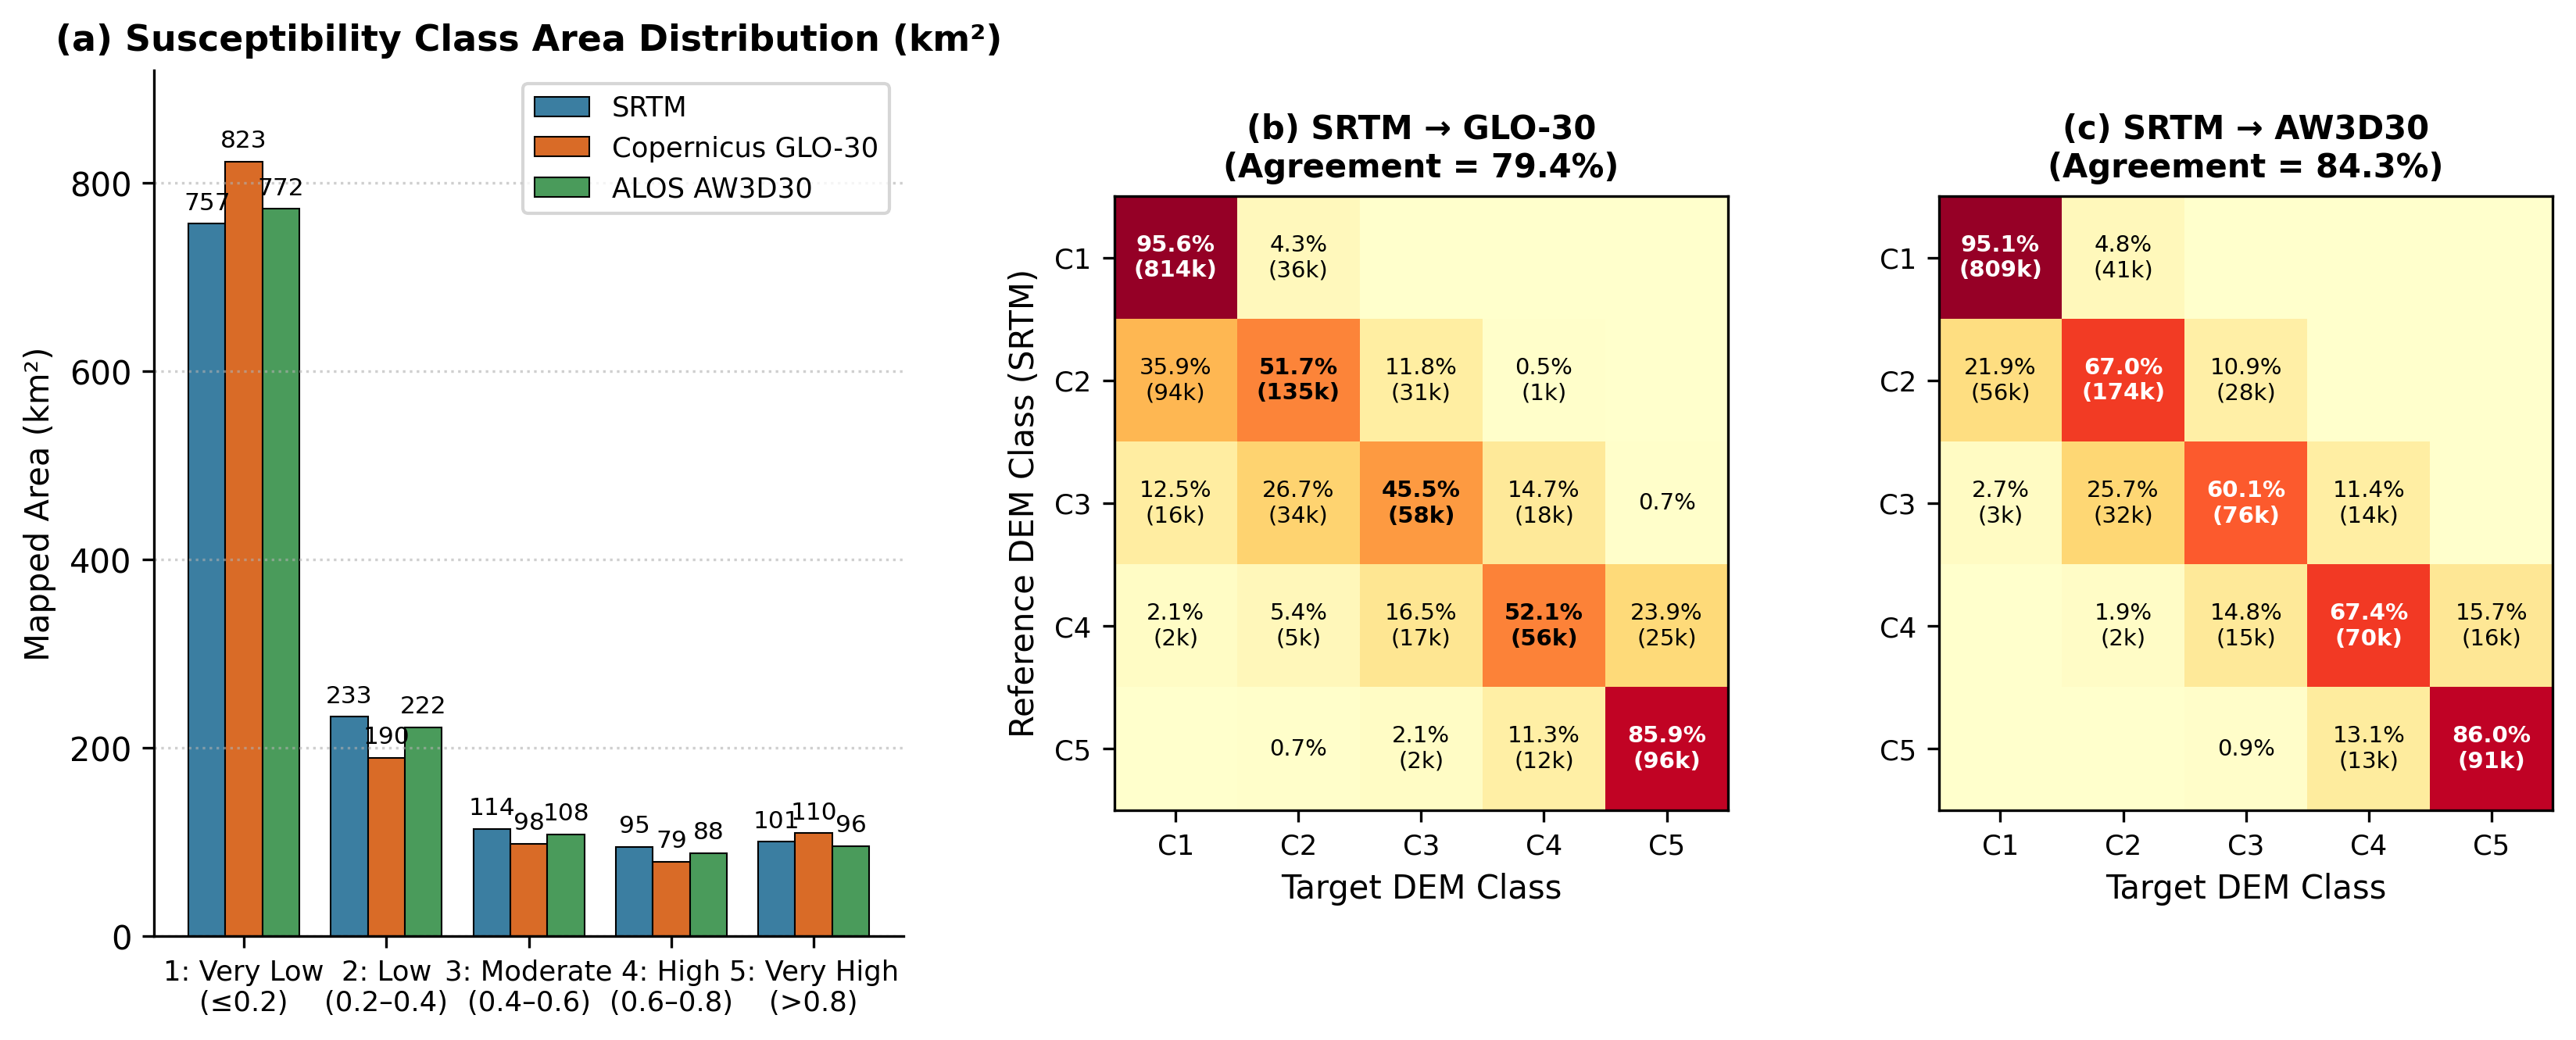
\includegraphics[width=0.94\textwidth]{figures/fig_spatial_sensitivity.png}
\caption{Sensitivitas spasial antarpeta kerawanan banjir: (a) luas area per kelas kerawanan ($\text{km}^2$); (b) matriks transisi kelas SRTM ke Copernicus DEM GLO-30; dan (c) matriks transisi kelas SRTM ke ALOS AW3D30.}
\label{fig:spatial-id}
\end{figure}

Hasil stratifikasi berdasarkan tutupan lahan ESA WorldCover (Tabel~\ref{tab:worldcover-id} dan Gambar~\ref{fig:agreement-id}) membuktikan bahwa sensitivitas spasial terhadap pergantian DEM sangat bergantung pada karakteristik penutup permukaan. Kelas tutupan pohon (\texttt{lc\_10}) memiliki kestabilan tertinggi (kesesuaian kelas $95{,}61\%\text{--}96{,}87\%$, $\overline{|\Delta p|} = 0{,}0113\text{--}0{,}0210$), diikuti kawasan terbangun (\texttt{lc\_50}, kesesuaian $87{,}19\%\text{--}91{,}18\%$). Sebaliknya, ketidaksepakatan spasial tertinggi terkonsentrasi pada semak belukar (\texttt{lc\_20}, kesesuaian $57{,}57\%\text{--}75{,}41\%$), mangrove (\texttt{lc\_95}, $62{,}64\%\text{--}74{,}87\%$), lahan terbuka/vegetasi jarang (\texttt{lc\_60}, $63{,}07\%\text{--}78{,}13\%$), dan lahan pertanian (\texttt{lc\_40}, $69{,}27\%\text{--}75{,}54\%$).

\begin{table}[!htbp]
\small
\centering
\caption{Stratifikasi sensitivitas spasial berdasarkan kelas tutupan lahan ESA WorldCover v200 pada ketiga pasangan produk elevasi.}
\label{tab:worldcover-id}
\begin{adjustbox}{max width=\textwidth}
\begin{tabular}{cl ccc ccc ccc}
\toprule
& & \multicolumn{3}{c}{\textbf{Rerata Selisih Probabilitas $\boldsymbol{\overline{|\Delta p|}}$}} & \multicolumn{3}{c}{\textbf{Tingkat Kesesuaian Kelas (\%)}} & \multicolumn{3}{c}{\textbf{Proporsi Berubah Kelas (\%)}} \\
\cmidrule(lr){3-5} \cmidrule(lr){6-8} \cmidrule(lr){9-11}
\textbf{Kode} & \textbf{Kelas WorldCover} & \textbf{SRTM--GLO30} & \textbf{SRTM--AW3D30} & \textbf{GLO30--AW3D30} & \textbf{SRTM--GLO30} & \textbf{SRTM--AW3D30} & \textbf{GLO30--AW3D30} & \textbf{SRTM--GLO30} & \textbf{SRTM--AW3D30} & \textbf{GLO30--AW3D30} \\
\midrule
10 & Tutupan pohon & 0,0210 & 0,0113 & 0,0170 & \textbf{95,61} & \textbf{96,78} & \textbf{96,87} & 4,39 & 3,22 & 3,13 \\
50 & Kawasan terbangun & 0,0514 & 0,0290 & 0,0373 & 87,19 & 91,18 & 90,77 & 12,81 & 8,82 & 9,23 \\
30 & Padang rumput & 0,0538 & 0,0300 & 0,0484 & 78,25 & 86,65 & 80,86 & 21,75 & 13,35 & 19,14 \\
80 & Badan air permanen & 0,0600 & 0,0405 & 0,0582 & 76,87 & 84,09 & 77,95 & 23,13 & 15,91 & 22,05 \\
90 & Lahan basah herba & 0,0609 & 0,0472 & 0,0574 & 72,46 & 78,29 & 74,24 & 27,54 & 21,71 & 25,76 \\
40 & Lahan pertanian & 0,0728 & 0,0526 & 0,0659 & 69,27 & 75,54 & 71,32 & 30,73 & 24,46 & 28,68 \\
60 & Lahan terbuka / veg.\ jarang & 0,0877 & 0,0478 & 0,0717 & 63,07 & 78,13 & 68,59 & 36,93 & 21,87 & 31,41 \\
95 & Mangrove & 0,0749 & 0,0493 & 0,0774 & 62,79 & 74,87 & 62,64 & 37,21 & 25,13 & 37,36 \\
20 & Semak belukar & \textbf{0,0943} & \textbf{0,0585} & \textbf{0,0915} & 59,07 & 75,41 & 57,57 & \textbf{40,93} & \textbf{24,59} & \textbf{42,43} \\
\bottomrule
\end{tabular}
\end{adjustbox}
\end{table}

\begin{figure}[!htbp]
\centering
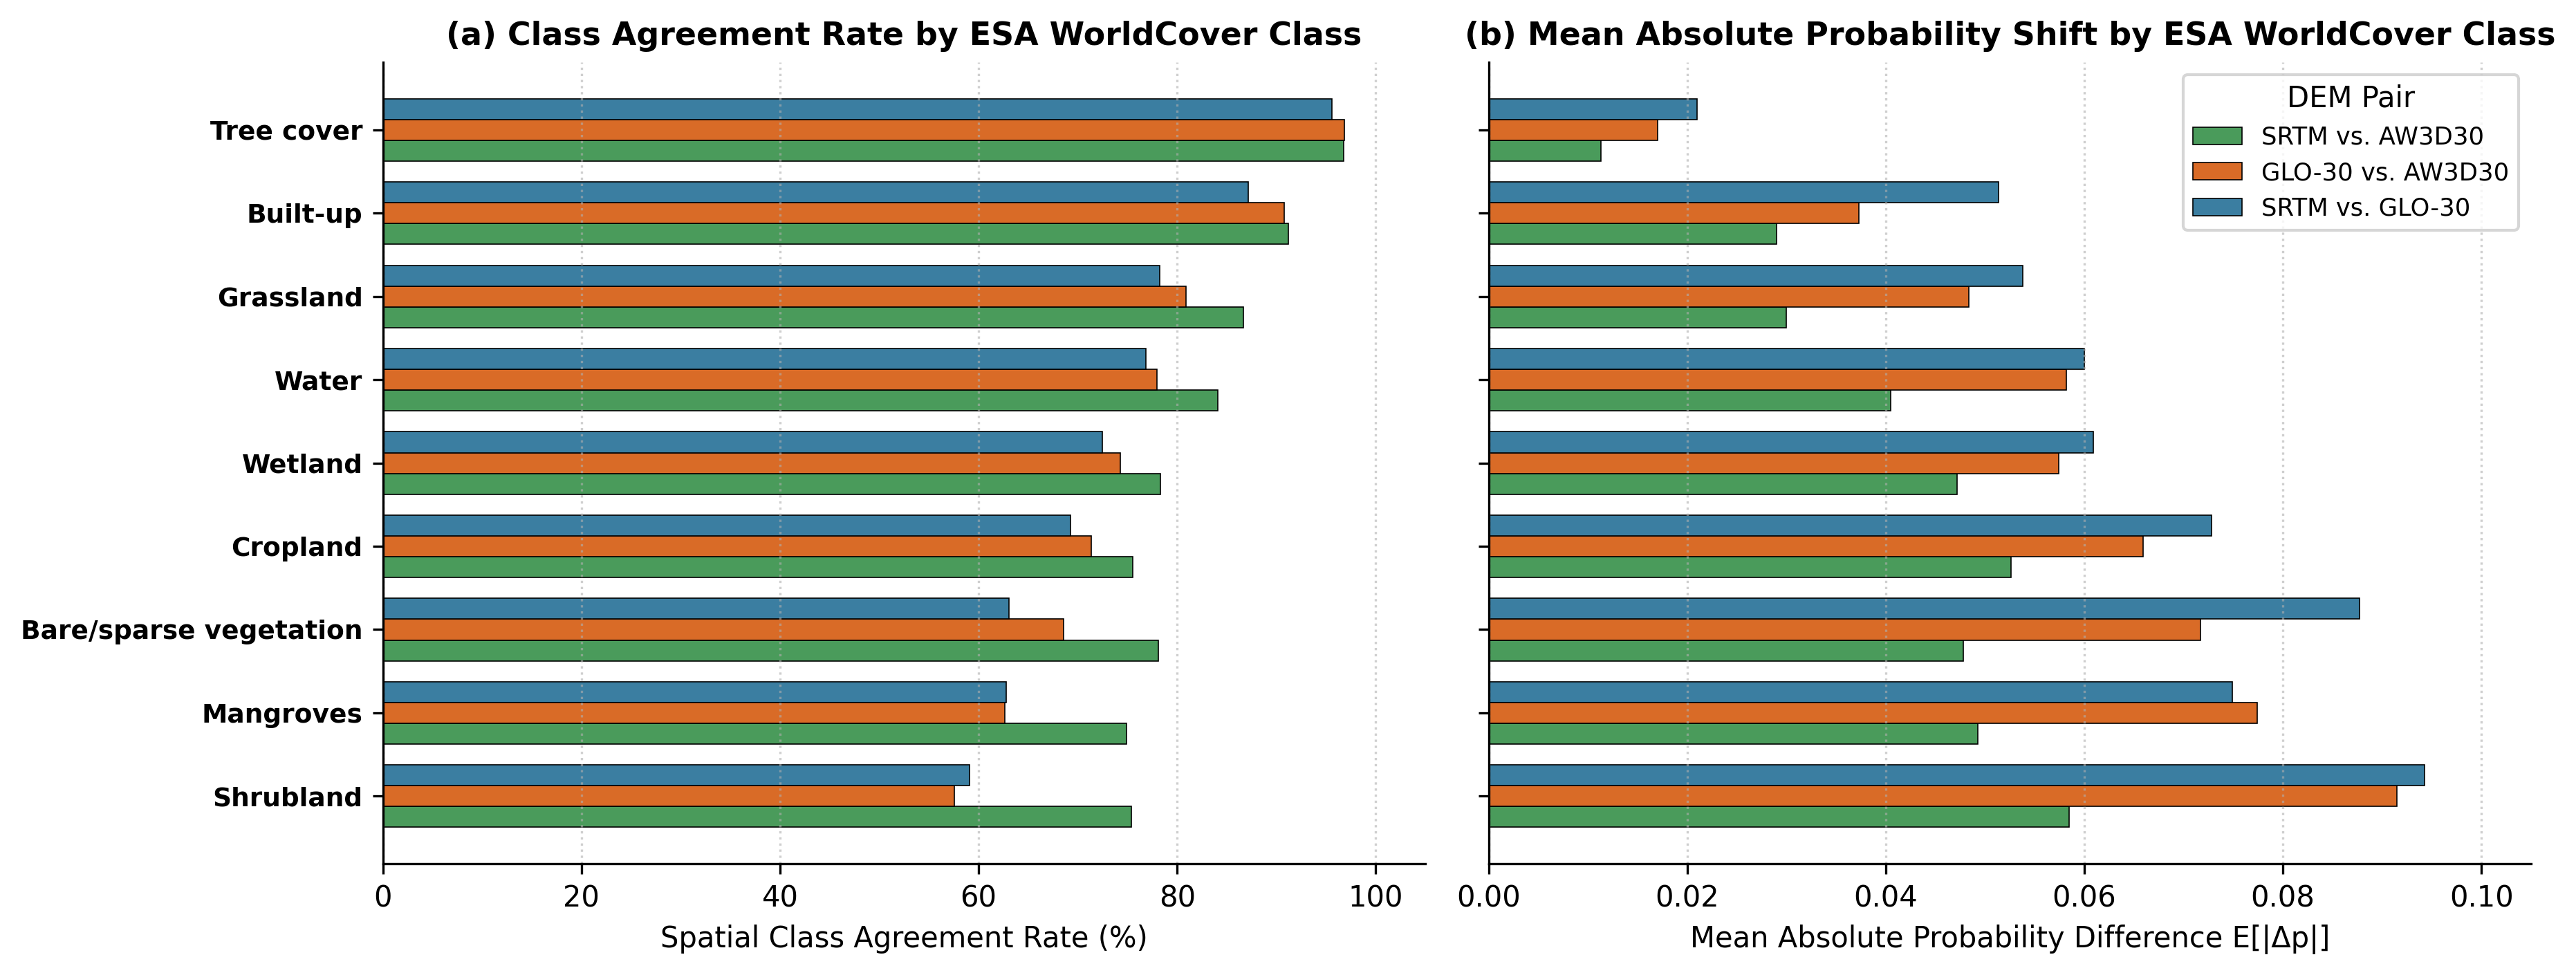
\includegraphics[width=0.94\textwidth]{figures/fig_agreement.png}
\caption{Stratifikasi sensitivitas spasial berdasarkan kelas tutupan lahan ESA WorldCover: (a) tingkat kesesuaian kelas (\%), dan (b) rerata selisih probabilitas absolut $\overline{|\Delta p|}$.}
\label{fig:agreement-id}
\end{figure}

Tabel~\ref{tab:moran-id} merangkum diagnostik autokorelasi spasial Global Moran's $I$ \cite{moran1950}. Pada $n = 5.956$ titik sampel (KNN $k=8$, $B=9.999$ permutasi), label banjir ($I = 0{,}677$) dan probabilitas OOF ($I = 0{,}877\text{--}0{,}886$) menunjukkan pengelompokan spasial yang kuat, sementara residual OOF ($r_i = y_i - \hat{p}_i^{\text{OOF}}$) masih menyisakan autokorelasi spasial positif signifikan ($I = 0{,}377$ pada SRTM, $0{,}355$ pada GLO-30, dan $0{,}364$ pada AW3D30; seluruhnya $p = 0{,}0001$) yang konsisten pada uji sensitivitas $k \in \{5, 8, 12\}$. Pada tingkat raster penuh pasca-masking AOI (Queen 8-tetangga, $B = 999$), ketiga peta probabilitas memiliki nilai Moran's $I$ sangat tinggi ($0{,}9531\text{--}0{,}9577$, $p = 0{,}001$).

\begin{table}[!htbp]
\small
\centering
\caption{Diagnostik Global Moran's $I$ pada prediksi/residual OOF ($n = 5.956$, KNN $k \in \{5,8,12\}$, $B = 9.999$) dan raster probabilitas GEE pasca-masking AOI (Queen 8-tetangga, $B = 999$).}
\label{tab:moran-id}
\begin{adjustbox}{max width=\textwidth}
\begin{tabular}{ll cccc ccc}
\toprule
& & \multicolumn{4}{c}{\textbf{Diagnostik Sampel OOF ($n = 5.956$, $E[I]=-0{,}000168$)}} & \multicolumn{3}{c}{\textbf{Raster Probabilitas AOI (Queen 8)}} \\
\cmidrule(lr){3-6} \cmidrule(lr){7-9}
\textbf{Konfigurasi DEM} & \textbf{Target} & \textbf{Moran's $\boldsymbol{I}$ ($k=8$)} & $\boldsymbol{z}$\textbf{-score} & \textbf{Resid.\ $\boldsymbol{I}$ ($k=5 / 8 / 12$)} & $\boldsymbol{p}$\textbf{-value} & \textbf{Piksel Valid ($n_{\text{used}}$)} & \textbf{Raster $\boldsymbol{I}$} & $\boldsymbol{z}$\textbf{-score ($p$)} \\
\midrule
Label Referensi $y_i$ & Banjir biner & 0,677 & 109,7 & --- & 0,0001 & --- & --- & --- \\
SRTM & $\hat{p}^{\text{OOF}}$ / $r^{\text{OOF}}$ & 0,886 / 0,377 & 143,6 / 61,4 & 0,418 / 0,377 / 0,345 & 0,0001 & 1.444.085 (0 isol.) & 0,9577 & 2.362,9 (0,001) \\
Copernicus GLO-30 & $\hat{p}^{\text{OOF}}$ / $r^{\text{OOF}}$ & 0,877 / \textbf{0,355} & 142,9 / \textbf{57,9} & \textbf{0,393} / \textbf{0,355} / \textbf{0,326} & 0,0001 & 1.444.085 (0 isol.) & 0,9531 & 2.351,7 (0,001) \\
ALOS AW3D30 & $\hat{p}^{\text{OOF}}$ / $r^{\text{OOF}}$ & 0,882 / 0,364 & 142,9 / 59,1 & 0,405 / 0,364 / 0,334 & 0,0001 & 1.429.580$^{\text{a}}$ (2 isol.) & 0,9544 & 2.252,0 (0,001) \\
\bottomrule
\multicolumn{9}{l}{\scriptsize $^{\text{a}}$Dua piksel terisolasi berderajat-0 ($n_{\text{valid}} = 1.429.582$) dikeluarkan dari penyebut standardisasi baris $S_0 = n_{\text{used}}$.}
\end{tabular}
\end{adjustbox}
\end{table}

\FloatBarrier

%==================================
\section{Pembahasan}\label{sec:pembahasan}

Temuan eksperimen terkontrol ini menjawab keempat rumusan masalah secara komprehensif. Pertama, walaupun SRTM, Copernicus DEM GLO-30, dan ALOS AW3D30 merepresentasikan struktur topografi makro yang selaras di Semarang--Demak, ketiganya berbeda secara sistematis di dataran aluvial pesisir. Interferometri radar bistatik pita-X lintasan tunggal pada Copernicus DEM GLO-30 menghasilkan permukaan dataran rendah dengan kemiringan lokal yang jauh lebih halus (median lereng titik banjir $0{,}28^\circ$) dibandingkan SRTM ($1{,}35^\circ$) dan ALOS AW3D30 ($0{,}96^\circ$) yang dipengaruhi derau fase radar pita-C maupun tekstur fotogrametri optik \cite{farr2007,tadono2016,esa_glo30,meadows2024}.

Kedua dan ketiga, kehalusan gradien lokal pada Copernicus DEM GLO-30 memberikan keunggulan daya diskriminasi yang konsisten pada Random Forest baik pada evaluasi \textit{holdout} ($\text{ROC-AUC} = 0{,}9404$) maupun validasi silang spasial 4-\textit{fold} ($\text{ROC-AUC} = 0{,}8899$). Analisis \textit{block bootstrap} 16 blok membuktikan pentingnya memperhitungkan autokorelasi spasial \cite{roberts2017,ploton2020}: keunggulan Copernicus GLO-30 terhadap SRTM ($\Delta\text{AUC} = +0{,}0155$) dan ALOS AW3D30 ($\Delta\text{AUC} = +0{,}0108$) tetap signifikan pada resampling tingkat blok, sedangkan selisih antara SRTM dan ALOS AW3D30 ($\Delta\text{AUC} = -0{,}0047$, CI 95\% $[-0{,}0096; +0{,}0013]$) terbukti marginal dan tidak berbeda nyata dari nol. Di sisi lain, meskipun selisih metrik evaluasi tingkat model berkisar $\sim 0{,}01\text{--}0{,}02$, perbandingan spasial pasca-masking AOI menunjukkan bahwa $15{,}7\%\text{--}20{,}6\%$ piksel valid berpindah kelas kerawanan ketika produk DEM diganti, dengan luas Kelas 5 (Sangat Tinggi) bergeser dari $100{,}58\text{ km}^2$ (SRTM) menjadi $95{,}93\text{ km}^2$ (AW3D30, $-4{,}6\%$) dan $109{,}63\text{ km}^2$ (GLO-30, $+9{,}0\%$), serta menyisakan autokorelasi spasial positif pada residual OOF (Moran's $I = 0{,}355\text{--}0{,}377$, $p = 0{,}0001$).

Keempat, stratifikasi ESA WorldCover menegaskan bahwa ketidakstabilan kelas antarpeta terkonsentrasi pada tutupan vegetasi pesisir dan pertanian berlereng landai---semak belukar, mangrove, lahan terbuka, dan lahan pertanian---di mana nilai probabilitas berada dekat batas ambang kelas dan interaksi sinyal sensor terhadap kanopi vegetasi rendah paling bervariasi \cite{meadows2024}. Selain itu, eksperimen diagnostik kami membuktikan bahwa perbaikan bias penyampelan kelas non-banjir pada mask JRC (\texttt{unmask(0)}) meningkatkan ROC-AUC spasial sebesar $\Delta\text{AUC} \approx 0{,}17$ (dari $\sim 0{,}70$ menjadi $0{,}870\text{--}0{,}890$), sepuluh kali lipat lebih besar daripada efek pergantian produk DEM. Adapun batasan penelitian ini meliputi penggunaan label proksi Sentinel-1 dari satu kejadian banjir (Maret 2024), dipertahankannya variabel hidrologi MERIT Hydro secara terkunci antarperlakuan, serta belum dimasukkannya data dinamis penurunan muka tanah dan pasang surut \cite{abidin2015,yuwono2024} yang direkomendasikan untuk penelitian multi-kejadian selanjutnya.

%==================================
\section{Kesimpulan}\label{sec:kesimpulan}

Berdasarkan eksperimen terkontrol sensitivitas produk elevasi global pada pemetaan kerawanan banjir berbasis Random Forest di wilayah pesisir Semarang--Demak, disimpulkan bahwa: (1) perbedaan karakteristik sensor dan datum vertikal antara SRTM, Copernicus DEM GLO-30, dan ALOS AW3D30 tercermin jelas pada elevasi median dan kemiringan lereng di dataran rendah pesisir; (2) ketiga produk mampu menghasilkan model kerawanan banjir berkinerja tinggi ($\text{Holdout AUC} = 0{,}932\text{--}0{,}940$; $\text{Spatial-CV AUC} = 0{,}870\text{--}0{,}890$); (3) Copernicus DEM GLO-30 unggul secara konsisten pada pengujian \textit{block bootstrap} dan replikasi 5-\textit{seed}, sementara pergantian DEM menggeser kelas kerawanan pada $15{,}7\%\text{--}20{,}6\%$ piksel valid AOI (mengubah luas Kelas 5 antara $95{,}93\text{ km}^2$ pada AW3D30 dan $109{,}63\text{ km}^2$ pada GLO-30) dengan autokorelasi residual OOF Moran's $I = 0{,}355\text{--}0{,}377$; dan (4) sensitivitas spasial tertinggi terjadi pada semak belukar, mangrove, lahan terbuka, serta lahan pertanian, sedangkan tutupan pohon dan kawasan terbangun paling stabil.

%==================================
\section*{Ketersediaan Data}
Notebook Google Earth Engine dan Python (\texttt{Flood\_DEM\_Sensitivity\_Notebook\_v28.ipynb} dan \texttt{T17\_Diagnostik\_Slope\_dan\_AOI\_v28.ipynb}), dataset sampel induk berimbang ($n = 5.956$), prediksi uji validasi silang spasial, tabel \textit{block bootstrap}, hasil replikasi 5-\textit{seed}, matriks transisi kelas, serta tabel stratifikasi ESA WorldCover tersedia secara terbuka untuk reproduksibilitas ilmiah.

\acknowledg{Penulis mengucapkan terima kasih kepada Program Studi Statistika dan Sains Data, FMIPA, Universitas Negeri Semarang atas dukungan akademik, serta kepada ESA, NASA/USGS, JAXA, dan tim Google Earth Engine atas penyediaan akses data geospasial terbuka.}

\FloatBarrier
\printbibliography[title={Daftar Pustaka}]

\end{document}
